\NeedsTeXFormat{LaTeX2e}
\documentclass[a4paper,12pt,
headsepline,           % Line between header and text
oneside,               % Single-sided
numbers=noenddot,      % No dots after chapter numbers
bibtotoc,              % Include bibliography in table of contents
BCOR15mm               % Binding correction
%,draft
]{scrbook}
\KOMAoptions{DIV=last} % Recalculate type area after loading package helvet

\pagestyle{headings}
\usepackage{blindtext}

% Helvetica as default font
\usepackage[scaled]{helvet}
\renewcommand{\familydefault}{\sfdefault} 

\usepackage{graphicx}
\usepackage[disable]{todonotes}
\usepackage{acronym}
\usepackage{orcidlink}
\usepackage{graphicx}
\usepackage{subcaption}
\usepackage{multirow}
\usepackage{booktabs}

% Bibliography with BibLaTeX
\usepackage[babel,german=quotes]{csquotes}
\usepackage[backend=bibtex8]{biblatex}
\bibliography{bibliography}

% Alternative with package option backend=biber and \addbibresource
% \usepackage[backend=biber]{biblatex}
% \addbibresource{bibliography.bib}

% For tables with fixed total width and variable column width
\usepackage{tabularx} 

% Special font styles
\usepackage{url}              % \url{http://...} in typewriter font
\usepackage{color}            % for setting colored text

\usepackage{amssymb, amsmath} % Packages for math environments and symbols

\usepackage{setspace}         % Package for various spacings, e.g. line spacing
%\onehalfspacing              % Only if required; it's quite large!!
\setlength{\parindent}{0pt}   % No indentation of the first line of paragraphs
\setlength{\parskip}{1.4ex plus 0.35ex minus 0.3ex} % Paragraph spacing, slightly variable

% Depth up to which headings are included in the table of contents
\setcounter{tocdepth}{3}      % Standard

% Examples of source code
\usepackage{listings}
\lstset{language=Java,
  showstringspaces=false,
  frame=single,
  numbers=left,
  basicstyle=\ttfamily,
  numberstyle=\tiny}

% Insert names etc. here
\newcommand{\fullname}{Dennis Huber}
\newcommand{\email}{dennis.huber@uni-ulm.de}
\newcommand{\titel}{Towards Robust Anomaly Detection in Univariate Time Series: A Multi-Algorithm Approach}
\newcommand{\jahr}{2024}
\newcommand{\matnr}{1164647}
\newcommand{\gutachterA}{Prof.\,Dr.\,Dr.\,Daniel Alexander Braun}
\newcommand{\gutachterB}{Prof.\,Dr.\,Friedhelm Schwenker}
\newcommand{\betreuer}{Sebastian Gottwald}

% Select the faculty here
%\newcommand{\fakultaet}{---  Adjust in the source code! ---}
\newcommand{\fakultaet}{Faculty of Engineering, Computer Science and Psychology}
%\newcommand{\fakultaet}{Mathematics and\\Economics}
%\newcommand{\fakultaet}{Medicine}
%\newcommand{\fakultaet}{Natural Sciences}

% Insert the institute here
\newcommand{\institut}{Institute for Neural Information Processing}

% Information that LaTeX writes into the PDF file
\pdfinfo{
  /Author (\fullname)
  /Title (\titel)
  /Producer     (pdfeTex 3.14159-1.30.6-2.2)
  /Keywords ()
}

\usepackage{hyperref}
\hypersetup{
pdftitle=\titel,
pdfauthor=\fullname,
pdfsubject={Diploma Thesis},
pdfproducer={pdfeTex 3.14159-1.30.6-2.2},
colorlinks=false,
pdfborder=0 0 0	% No box around links!
}

% Hyphenation rules
\hyphenation{hy-phen-ation}

\begin{document}
\frontmatter

% Title page
\thispagestyle{empty}
\begin{addmargin*}[4mm]{-10mm}

\hfill

\includegraphics[height=1.8cm]{images/logo_uulm_sw.png}\\[1em]

{\footnotesize
%{\bfseries Universität Ulm} \textbar ~89069 Ulm \textbar ~Germany
\hspace*{115mm}\parbox[t]{35mm}{\bfseries 
\fakultaet\\
\mdseries \institut}\\[2cm]

\parbox{140mm}{\bfseries \LARGE \titel}\\[2.5em]
{\footnotesize Thesis submitted to the University of Ulm}\\[3em]

{\footnotesize \bfseries Submitted by:}\\
{\footnotesize \fullname\, \orcidlink{0009-0002-5723-9699}\\ \email}\\ \matnr\\[2em]
{\footnotesize \bfseries Supervisors:}\\                     
{\footnotesize \gutachterA\\ \gutachterB}\\[2em]
{\footnotesize \bfseries Advisor:}\\ 
{\footnotesize \betreuer}\\\\
{\footnotesize \jahr}
}
\end{addmargin*}


% Imprint
\clearpage
\thispagestyle{empty}
{ \small
  \flushleft
  Version \today \\\vfill
  \copyright~\jahr~\fullname\\[0.5em]
% If you want to provide your work under a free license, you can include the next line in your code. Please note that you need the necessary rights for all content, including included illustrations! When publishing your dissertation, please ensure that the license text does not contradict the information in the metadata of the publication platform used. More information about the Creative Commons licenses can be found here: https://creativecommons.org/licenses/
%This work is licensed under the Creative Commons Attribution 4.0 International (CC BY 4.0) License. To view a copy of this license, visit \href{https://creativecommons.org/licenses/by/4.0/}{https://creativecommons.org/licenses/by/4.0/} or send a letter to Creative Commons, 543 Howard Street, 5th Floor, San Francisco, California, 94105, USA. \\
  Typesetting: PDF-\LaTeXe
}

% From here, slightly larger line spacing
\setstretch{1.2}

\tableofcontents

\mainmatter
\chapter{Introduction}
\label{ch:introduction}

\todo{Versuchen ein universelles Beispiel zu finden, dass sich durchzieht}
\todo{gesamtes Dokument: Trennen Algorithm vs. Method}

\textit{Anomaly Detection (AD)} has been around since we started collecting data. Early scientists relied on simple observations and charts to look for anything abnormal. For instance, in the 16th century, astronomers like Tycho Brahe observed the night sky with high precision, recording unusual celestial events. When Brahe observed a supernova, it marked a significant anomaly in his records that contradicted the belief, the night sky would not change and propelled advancements in astronomy \cite{Decourchelle2017}.

Today, we can leverage additional tools, like statistics, \textit{Machine Learning (ML)} and \textit{Artificial Intelligence (AI)} to enhance our ability to detect anomalies. These technologies allow us to analyze much bigger amounts of data, revealing patterns and insights that would have been hidden to the naked eye.

As we reflect on the journey of AD from the precise charts of Brahe to the powerful algorithms today, it becomes clear that detecting and understanding anomalies is not just about identifying outliers. It is about discovering the abnormal in our data and learning from it, ultimately driving innovation across various fields.

In this master thesis, we want to continue this journey by providing insights into the vast variety of AD techniques. Past research has shown that the great diversity of patterns still asks for the careful eye of researchers to thoughtfully apply the right technique to their data. Just like Brahe, modern scientists need to carefully analyze their data and have a deep understanding of the tools they use. We want to support this process by mapping existing techniques from different fields to emerging patterns in time series data to provide guidelines for picking the appropriate tool.

To achieve this and contribute to this journey, we start by delivering the foundations for understanding the dataset. We introduce the characteristics and specialties of time series data and explain common modeling techniques. We further define anomalies and categorize them so the analyst know what to expect. The last brick of the foundation is the explanation of AD techniques. In this section, a taxonomy is introduced to categorize the different approaches and develop an overview. Before we introduce the current state of the art from the literature, we discuss the problem this master thesis is dealing with and define what is in- and outside its scope. 

The literature review introduces decomposition and feature extraction on time series data before jumping to a thorough analysis of AD algorithms. The comprehensive review of different approaches towards AD, their strengths and weaknesses forms a great part of the added value of this paper to the journey of AD

%\section{Background and Motivation}
% why good to detect anomalies
%The goal of this master thesis is to provide guidelines to the readers, so they can make an informed decision on which algorithm suits their use-case. As mentioned above, different algorithms have different strengths and weaknesses depending on the given data characteristics. For instance, deep learning algorithms with \textit{Long-Short-Term Memory (LSTM)} can capture patterns across many time steps, while . Such incorporated structures must be understood to map them to the expected anomalies. But, to perform such a mapping, a deep dive into the different types of anomalies is essential to understand their diversity, which is often much more complex than breaking a simple threshold. Within the scope of this work, the discussed data structure in which the anomalies appear are time-series. So in order to conclude the path towards the final guidelines, we start by understanding these special data structures.

\section{Time Series}
\label{sec:time_series}
\todo{einigen auf "time series data"/ "time series"/ "time-series"}
% Introduction to time series
A time series is a sequence of data points recorded at discrete time during specific intervals. The data points are often real numbers, which are typically spaced uniformly. The primary characteristic that distinguishes time series data from other types of sequential data is the temporal order, which is extremely common when observing real world phenomena \cite{Cryer2009}. 

We follow a general definition of time series \cite{Kreis2006}:
\begin{equation}
    \label{eq:time_series}
    X = (X_t : t \in T), \quad T = \mathbb{Z},
\end{equation}

Where $t$ denotes the time index and $X_t$ are real-numbered data points, which can be multidimensional $X_t \in \mathbb{R}^n$. We further note that $T = \mathbb{N}$ is another common definition of time series as it usually starts at a specific point in time (e.g. $t=1$). However, $T=\mathbb{Z}$ assumes an infinite past and does not require special treatment of an initial value.

% univariate, equidistant
In Equation \ref{eq:time_series} we assume that the time series is \textit{equidistant}. This means that the data points $X_t$ were collected at regular, uniformly spaced intervals. This regularity simplifies the analysis, as many time series models assume equidistant intervals for their mathematical formulations \cite{Chatfield2003}.
Non-equidistant time series are rare but can occur in domains like healthcare, where patient visits may not follow a regular schedule. Analyzing non-equidistant time series often requires specialized techniques that can handle the irregular spacing of data points.
Formally, if the time series is equidistant, then for all $t$ and $t'$ where $t \neq t'$, the time intervals $\Delta t = t_{k+1} - t_k$ are constant.

The formulation in Equation \ref{eq:time_series} can also describe one-dimensional data points $X_t \in \mathbb{R}$, which makes $X$ a \textit{univariate} time series. In the multidimensional case above, it is called \textit{multivariate}.
Univariate time series record one variable at a time, such as a stock price \cite{Sinha2022}. Multivariate time series, on the other hand, record multiple variables simultaneously, which can be of the same type or a mixture of different data types \cite{Chandola2009}. For example in economics, analysts might consider variables like GDP, inflation, and commodity price together \cite{Verstyuk2019}.
In the field of AD, univariate time series can often be handled by simpler models as they are less computationally expensive, while multivariate models can capture the interdependencies between variables, offering a more comprehensive understanding of a system \cite{Chandola2009}.

To complete the justification of using Equation \ref{eq:time_series} as our definition of time series, it should be mentioned that there are also continuous time series definitions. However, the concept of continuous time series comes into play in a theoretical or modeling context. Since this work deals with observations recorded at distinct, separate time points, Equation \ref{eq:time_series} for discrete time series is considered adequate.

\subsection{Real-World Examples}
% - Where are time series coming from
Time series are ubiquitous and can be found across various domains, like finance, meteorology or healthcare. 
In finance, stock prices are one of the most common examples. They are recorded at regular intervals, such as daily or minute-by-minute, and are used to analyze market trends and make investment decisions. 
In meteorology, temperature readings taken at regular intervals (e.g., hourly) form a time series that can be analyzed to understand weather patterns, climate change, and seasonal variations. 
In healthcare, heart rate monitoring involves recording heart rates at regular intervals, often in real-time, to monitor a patient’s health condition and manage chronic diseases. 
In each of these examples, the overall goal is to analyze patterns, detect anomalies or forecast future values based on the recorded time series data. A significant aspect of \textit{time series analysis (TSA)}.


\subsection{Analysis and Characteristics}

\begin{figure}
    \centering
    
\includegraphics[width=0.5\linewidth]{images/placeholder.png}
    \caption{Run Chart of a Time Series}
    \label{fig:run_chart_example}
\end{figure}

% - characteristics of time series
In real world applications, such as the examples given above, time series are often captured over longer periods of time, which leads to long sequences. The straight forward approach is to plot such sequences in a run chart, like in Figure \ref{fig:run_chart_example}, to get meaningful insights into the data. With longer sequences, however, it can be difficult to discover patterns within the plot. The goal of TSA is to use the right techniques to describe past patterns to detect, eliminate or forecast past and future patterns \cite{Vishwas2020}. 

Someone could easily imagine how this could be translated to AD. In fact, AD is a subset of TSA, which uses its techniques to model a normal behavior and distinguish the unusual. For this reason, this section only covers the time series characteristics derived from TSA as modeling is covered in Chapter \nameref{ch:literature_review}.

Understanding the different characteristics within time series is essential for an effective analysis. Generally, time series can be analysed in the \textit{time domain} or the \textit{frequency domain}, which are not mutually exclusive \cite{Shumway2017}.
The time domain approach covers the temporal dynamics of the data, such as the relationship between current values and past values. It excels in understanding direct temporal relationships and forecasting.
The frequency domain approach covers the cyclical behavior in the data. Instead of looking at how past values influence future ones, it examines the series in terms of periodic cycles or oscillations. It is particularly useful for detecting regularities and periodicities that might not be obvious in the time domain.
Generally speaking, while the time domain is concerned with "when" changes happen, the frequency domain is focused on "how often" changes happen.

Shumway and Stoffer \cite{Shumway2017} formulated a set of time series characteristics around these domains using real experimental data:

% Wichtig weil kommt zur Sprache in def. anomaly
\paragraph{Temporal correlation} is one of the primary characteristics of time series data, meaning that an observation $X_(t')$ can be highly dependent on its previous observations where $t<t'$. This poses a challenge for traditional statistical methods, which often assume independence among observations \cite{Student1908, PEARSON1920, Fisher1992, Russell2020, Edgeworth}. However, in certain contexts, the \textit{Markov property} can be applied, suggesting that the future state of a process depends only on its present state and not on its past states. This simplifies the analysis by allowing models to focus on the most recent observations. Measures such as \textit{autocovariance} or \textit{autocorrelation} (explained in \ref{}) help models to account for temporal correlations by capturing the dynamic nature of the data while following the Markov property when appropriate.

\begin{figure}
    \centering
    % First Row of Subfigures
    \begin{subfigure}[b]{0.45\textwidth}
        \centering
        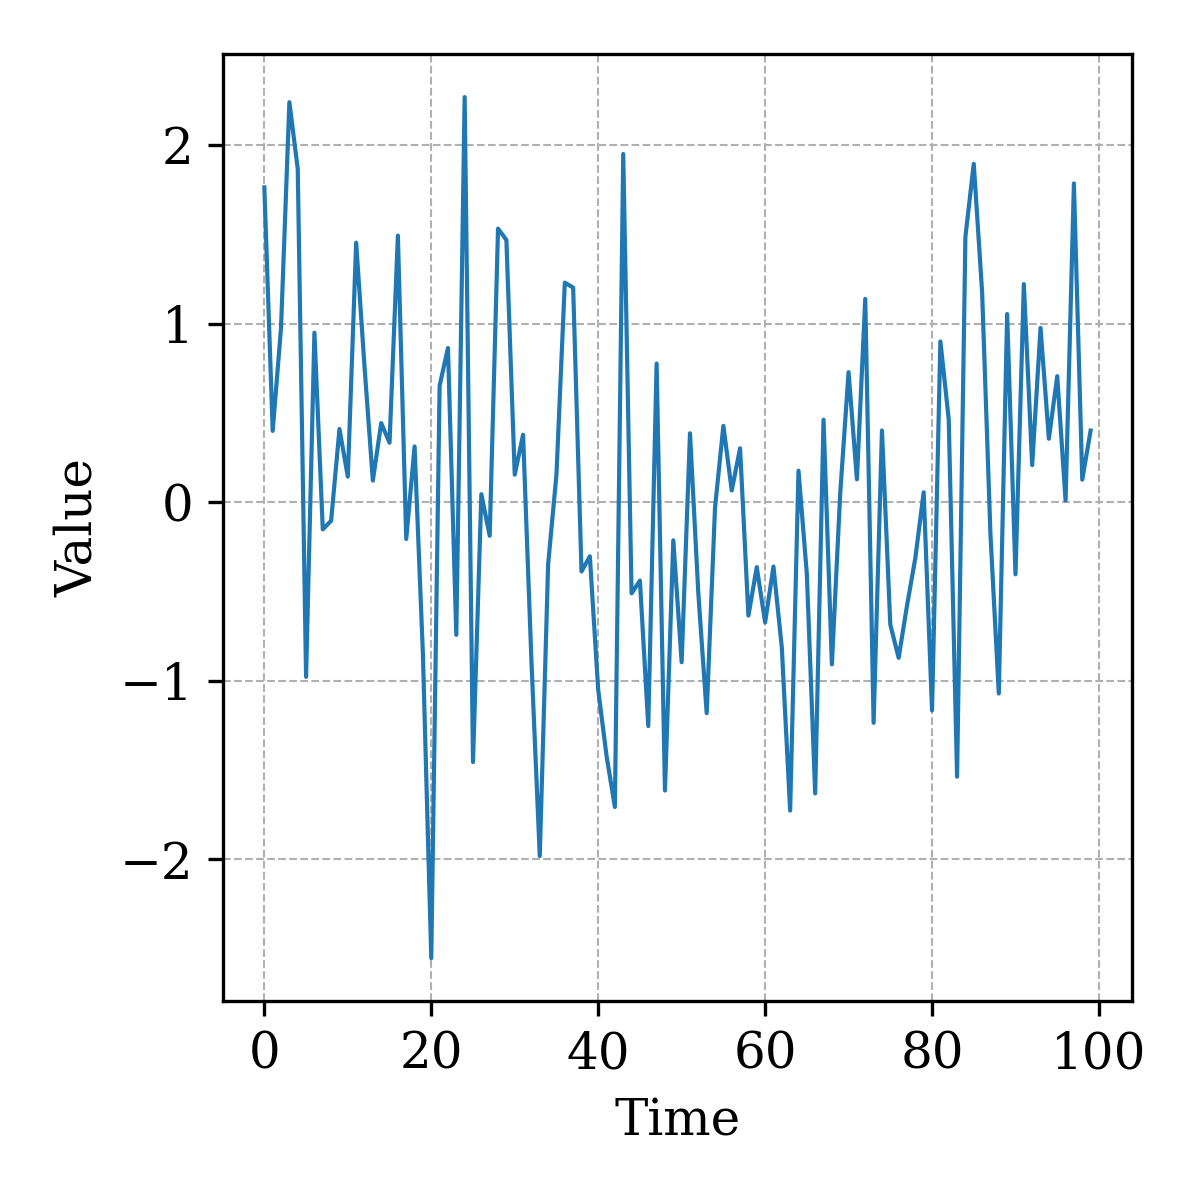
\includegraphics[width=\textwidth]{plots/stationarity_plots/stationary_time_series.png}
        \subcaption{Stationary Time Series}
        \label{fig:stationary}
    \end{subfigure}
    \hfill
    \begin{subfigure}[b]{0.45\textwidth}
        \centering
        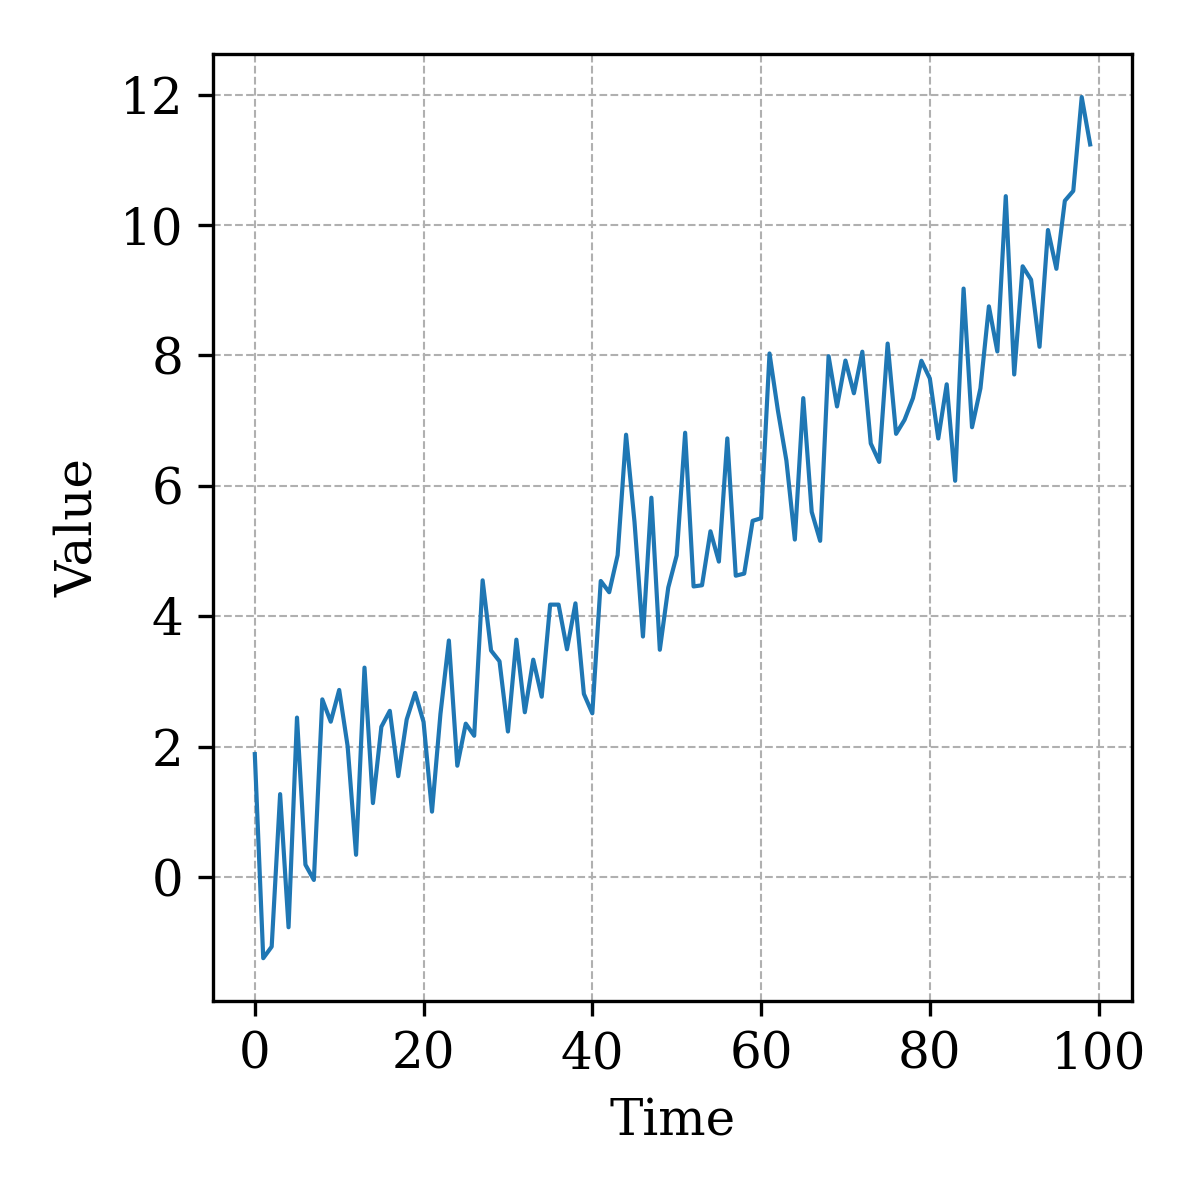
\includegraphics[width=\textwidth]{plots/stationarity_plots/nonstationary_time_dependent_mean.png}
        \subcaption{Non-Stationary Series with Time-Dependent Mean}
        \label{fig:nonstationary_mean}
    \end{subfigure}
    % Second Row of Subfigures
    \vskip\baselineskip
    \begin{subfigure}[b]{0.45\textwidth}
        \centering
        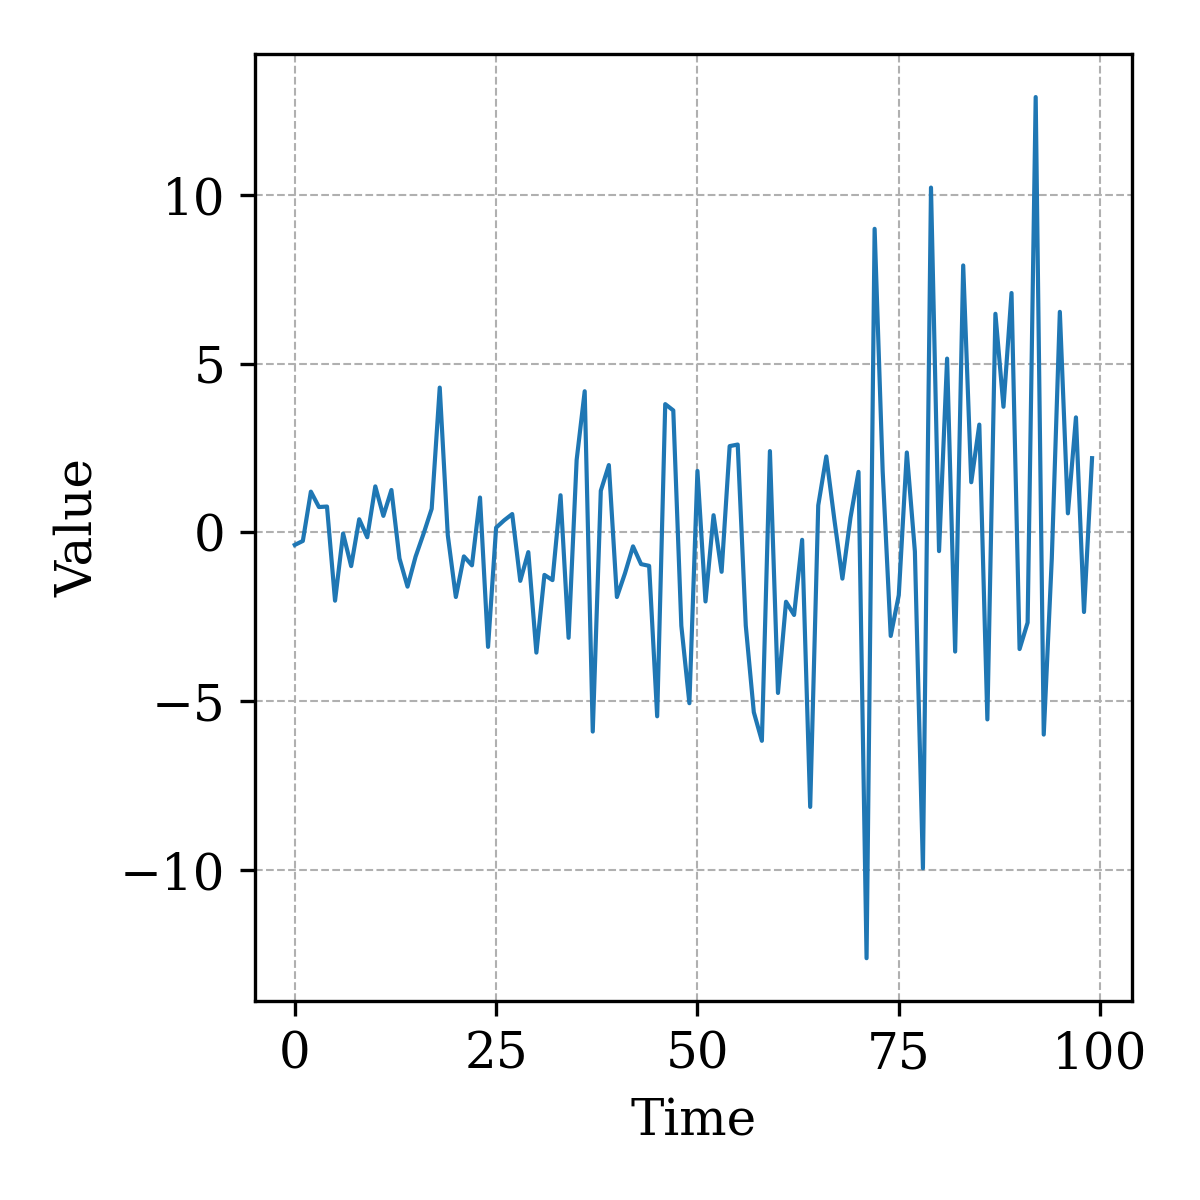
\includegraphics[width=\textwidth]{plots/stationarity_plots/nonstationary_time_dependent_variance.png}
        \subcaption{Non-Stationary Series with Time-Dependent Variance}
        \label{fig:nonstationary_variance}
    \end{subfigure}
    \hfill
    \begin{subfigure}[b]{0.45\textwidth}
        \centering
        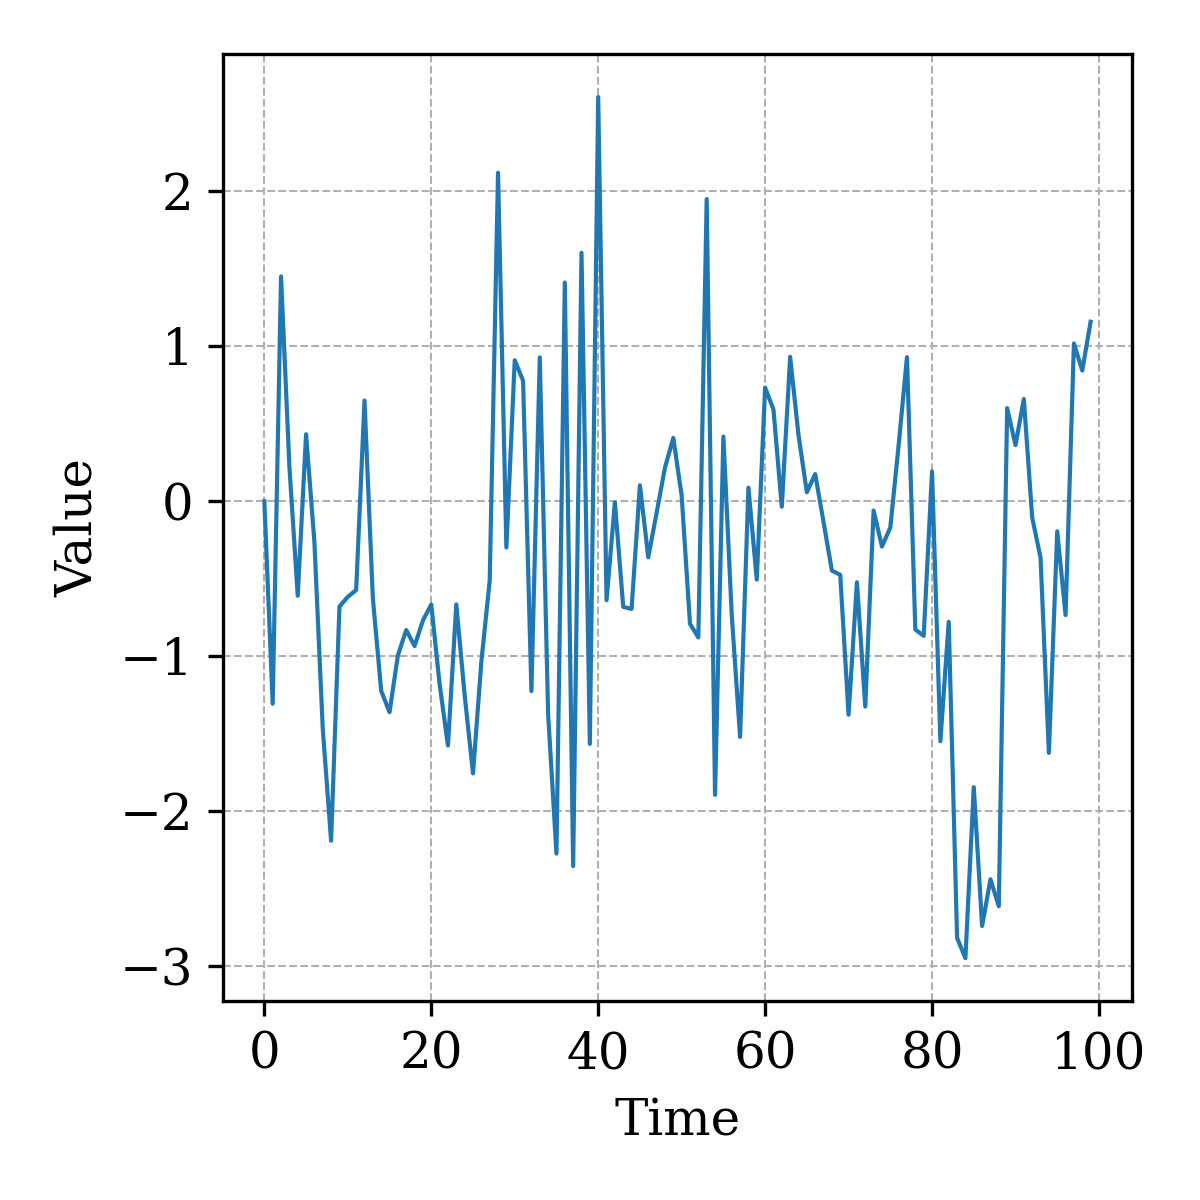
\includegraphics[width=\textwidth]{plots/stationarity_plots/nonstationary_time_dependent_covariance.png}
        \subcaption{Non-Stationary Series with Time-Dependent Covariance}
        \label{fig:nonstationary_covariance}
    \end{subfigure}
    \caption{Comparison of Stationarity and Non-Stationarity in Time Series}
    \label{fig:stationarity_comparison}
\end{figure}

\paragraph{Stationarity} refers to a characteristic where statistical properties such as mean and variance remain constant over time, like in Figure \ref{fig:stationary}. 
However, time series can show trend, seasonality or cyclic components, which introduce non-stationarity. The key concept is to perform a transformation and achive stationarity, as non-stationary data can lead to misleading statistical inferences and poor forecasting performance \cite{Hamilton1989}. 

A \textit{trend ($T$)} refers to a long-term movement, indicating an overall increase or decrease in the data over an extended period. It is usually represented by the mean rate of change over time and, therefore, is a type of non-stationarity \cite{Vishwas2020}. In Figure \ref{fig:nonstationary_mean} we illustrated a linear, upward trend, which shows in the graph and is indicated by a linearly increasing mean. Generally, a trend pattern can also be nonlinear, which makes its identification difficult.

\textit{Seasonal ($S$)} and \textit{Cyclic ($C$)} components involve fluctuations, rather than long-term movements. Seasonalities are regular patterns with a fixed and predictable duration, like a temperature increase and decrease during the day. Cyclic patterns, in contrast, are not as regular or predictable, like economic cycles. Both patterns can introduce all three types of non-stationarities from Figure \ref{fig:stationarity_comparison} to different degrees. Differentiating between the two is crucial to transform the non-stationarities accordingly \cite{Box2013}. 

\paragraph{Irregularities ($I$)} are unexpected variations or random noise within the data. They appear irregularly but usually do not effect stationarity.

We take Equation \ref{eq:time_series} and \textit{decompose} the time series $X_t$ at any time $t$ to a linear (Equation \ref{eq:linear-decomposition}) and non-linear (Equation \ref{eq:non-linear-decomposition}) model of its components \cite{Vishwas2020}:

\begin{equation}
\label{eq:linear-decomposition}
    X_t = T_t + S_t + C_t + I_t
\end{equation}
\begin{equation}
\label{eq:non-linear-decomposition}
    X_t = T_t \cdot S_t \cdot C_t \cdot I_t
\end{equation}

After decomposing the time series using such a model, each component can be tackled individually to achieve stationarity. 


\section{Anomalies}
% - What are anomalies: explain anomaly; anomaly vs. outlier; anomaly detection KURZ erklären
We introduced trend, seasonality and cycle patterns above. With the knowledge about their nature and by taking a look at the Figure \ref{fig:stationarity_comparison} again, the sudden changes already appear anomalous. But are these patterns already \textit{anomalies}?

In the field of anomalies in time series, defining an anomaly is both crucial and complex. An anomaly, in a general contexts, is something that deviates significantly from the norm, raising suspicions about its origin or nature \cite{mw:anomaly}. This definition can be put into the context of statistics. Here, data points that are far from the distribution are considered \textit{outliers}. However, it is difficult to determine how far a data point needs to deviate from the distribution in order to be considered an anomaly. Hawkins \cite{Hawkins1980} refines this by saying that an outlier has to deviate to such an extend that it was caused by a different mechanism other than random error in order to be an anomaly. 

This definition is very close to the terms \textit{abnormal} \cite{cb:abnormal} or \textit{deviant} \cite{cb:deviant}, which is why they are often used interchangeably \cite{Whitehead1995}. In this work we use the term \textit{anomaly} exclusively to avoid confusion. In the literature review in Chapter \ref{ch:literature_review}, other terms might appear, which are used by the authors of the presented paper. This helps to link the information to the origin paper but it is always made clear that it is a synonym of "anomaly".

In some contexts, \textit{novelty} \cite{cb:novelty} is used as a synonym for anomaly. However, in the field of AD it is important to differentiate between the two terms. For instance, a smart watch user lends his device to a friend. Due to novel arm movements, the smart watch detects them as anomalies and the watch stops working properly. This example shows how novelties need to be distinguished from anomalies to become part of the system's normal behavior, which is often not trivial.
\todo{Einbauen: anomaly = imbalanced datasets per definition}

Going back to the initial question, we now answer that the time series follows a normal behavior and significant deviations are considered anomalies. Decomposition describes the normal behavior in a more refined way and offers better comparison to define the anomalous.  

\begin{figure}
    \centering
    \begin{subfigure}[b]{0.45\textwidth}
        \centering
        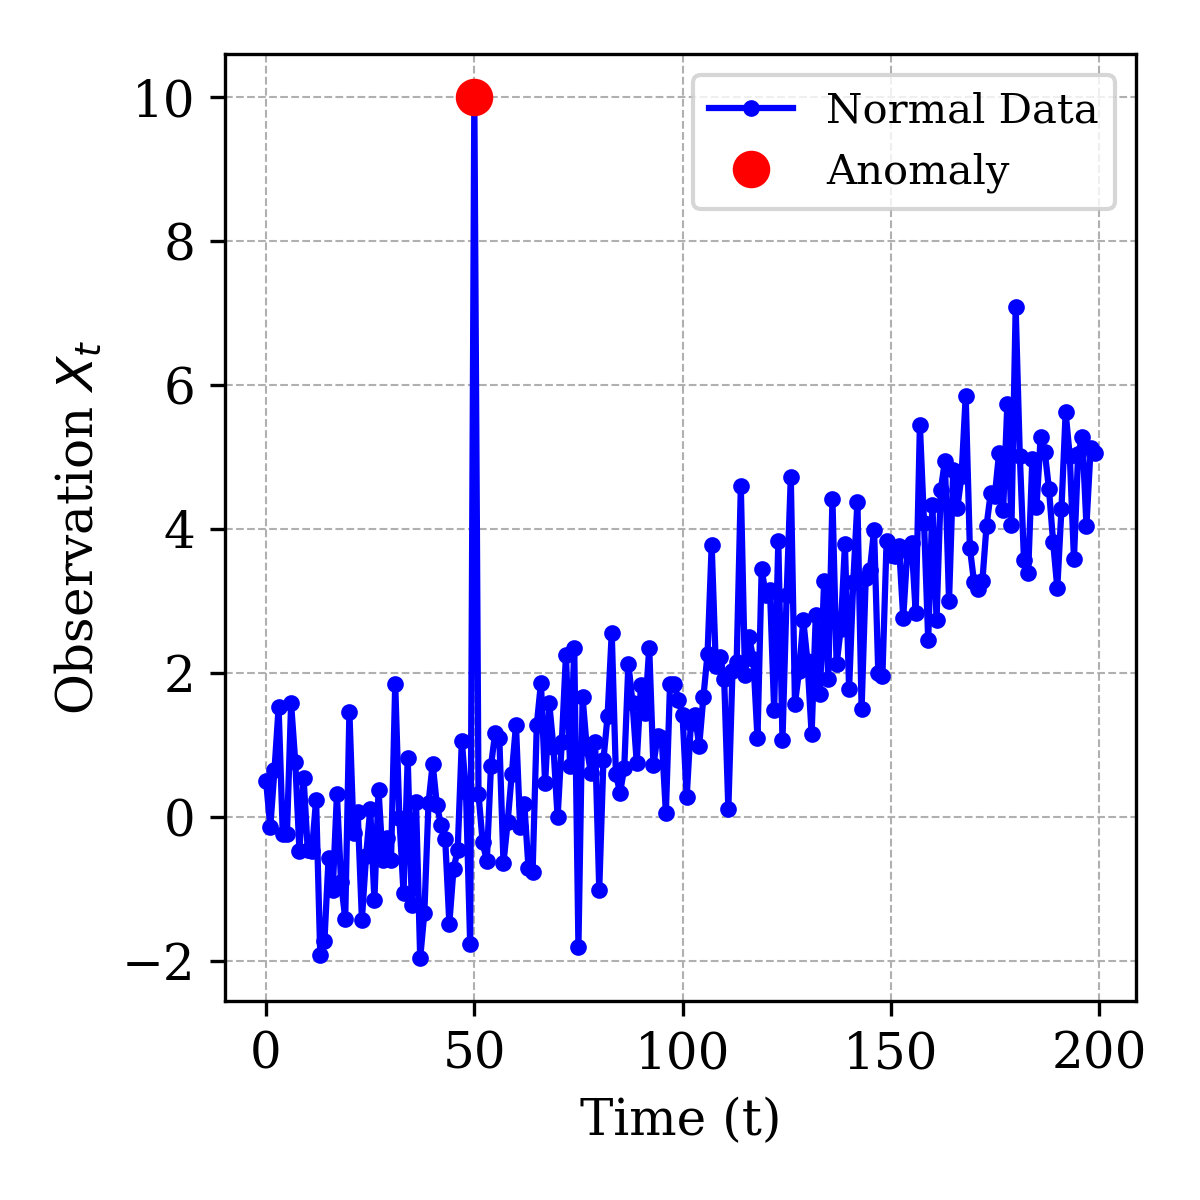
\includegraphics[width=\textwidth]{plots/temporal_correlation_plots/run_chart_with_anomaly.png}
        \subcaption{Run Chart of $X$}
        \label{fig:run_chart}
    \end{subfigure}
    \hfill
    \begin{subfigure}[b]{0.45\textwidth}
        \centering
        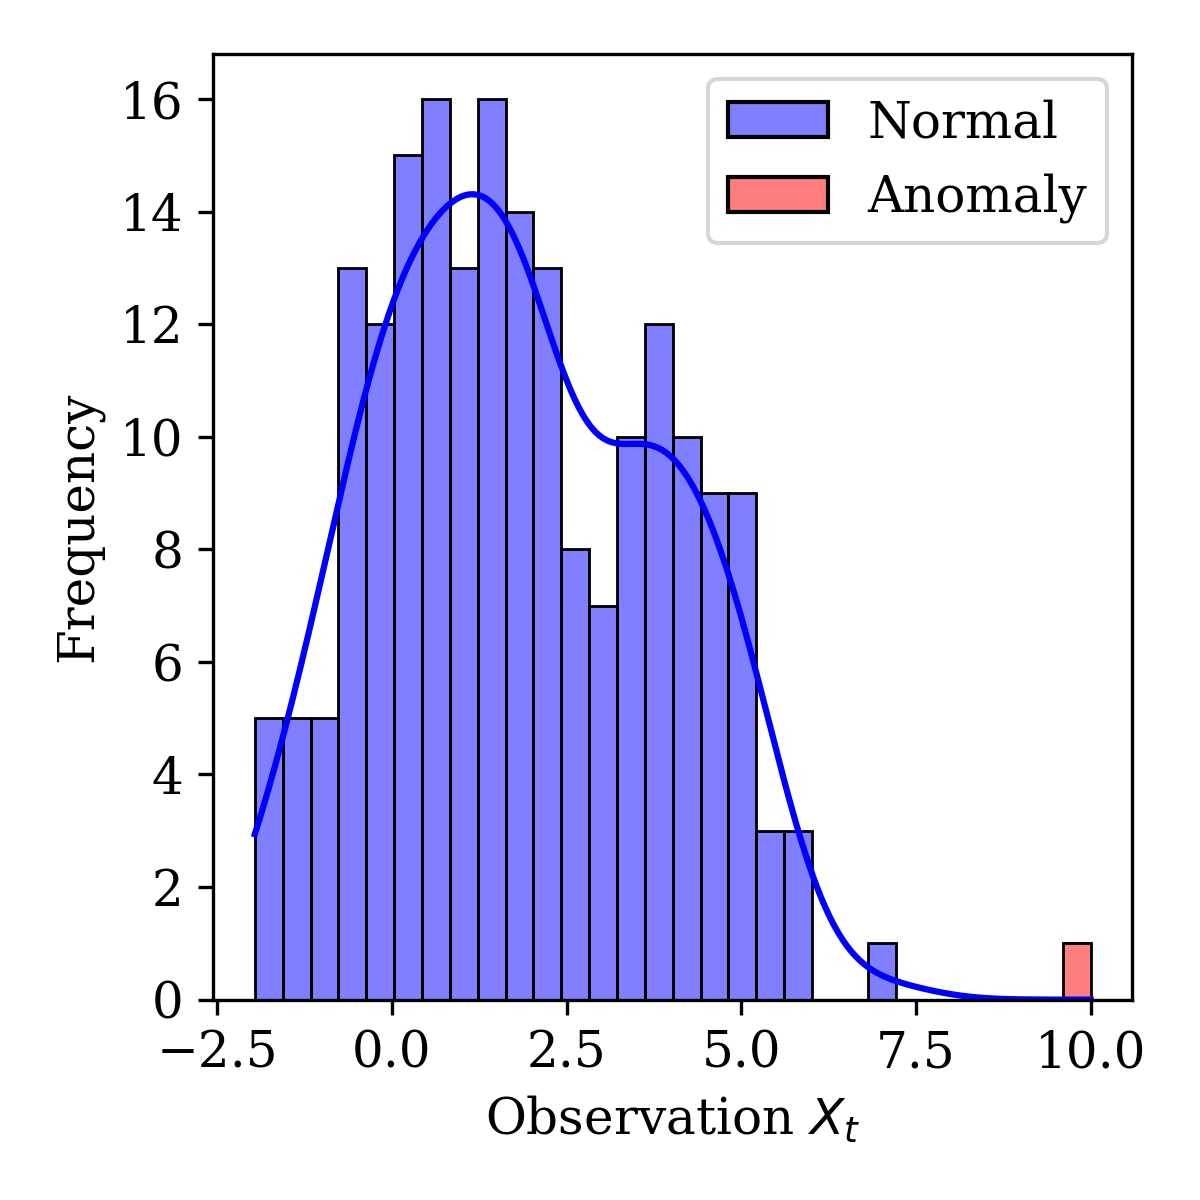
\includegraphics[width=\textwidth]{plots/temporal_correlation_plots/distribution_chart_with_anomaly.png}
        \subcaption{Distribution of all $X_t \in X$}
        \label{fig:distribution_chart}
    \end{subfigure}
    
    \caption{Time Series with Extremum and Trend Anomaly}
    \label{fig:temporal_correlation_comparison}
\end{figure}
Anomalies in time series data also differ from other data types, where it might sorely depend on the underlying statistical properties and distributions. We observe Figure \ref{fig:run_chart}, where the data points $X_t$ are plotted along a time axis in sequential order $X$. We notice a spike around $t=50$, which clearly strikes as an anomaly. We also observe a following upward trend, which is not visible for $t<50$ and should also be considered anomalous. If we observe Figure \ref{fig:distribution_chart}, where we neglected the temporal order by plotting the distribution of all $X_t$, we can detect the anomaly $X_{50} = 10$ as it is outside the distribution. However, the distribution does not show the trend anomaly as it simply caused it to skew. 

This example shows that the importance of respecting the temporal correlation when detecting anomalies in time series. It also shows that there are different types of anomalies. Chandola et al. \cite{Chandola2009} formulates three anomaly types:

\begin{itemize}
    \item \textit{Point anomalies} are data instances, which significantly differ from the rest of the data, like the anomalous data point $X_{50}$.
    \item \textit{Contextual anomalies} are only considered anomalous in a specific context but may appear normal otherwise, like the trend anomaly for $t>50$. These anomalies require the definition of a context as an overall trend could also be considered a component of the time series' normal behavior. 
    \item \textit{Collective anomalies} are groups of related data instances, which appear anomalous relative to the entire dataset, even if some instances do not appear anomalous. For example, a consistent sequence of low values in an electrocardiogram reading could signify a heart condition, even though individual low readings may be normal.
\end{itemize}

Contextual and collective anomalies show that the AD is no trivial task. We highlight the importance of defining the normal behavior to improve the detection of the abnormal. We introduced the concepts of modeling and decomposing time series to better understand and transform the normal behavior. Using this refined definition of our normal behavior, we can use a more typification of anomalies by introducing nine \textit{anomaly kinds} \cite{Schmidl2022}:

\begin{itemize}
    \item \textit{Amplitude Anomalies} occur when one or multiple consecutive values deviate significantly in magnitude from the norm. This type of anomaly is characterized by spikes or drops that stand out from the typical range of values. They indicate potential errors, sudden changes in conditions, or unexpected events.

    \item \textit{Extremum Anomalies} refer to data points that represent extreme single values, either as unusually high peaks or low troughs within the data. These anomalies can signify exceptional events, such as system overloads, failures, or extreme external conditions affecting the data. The peak $X_50$ in Figure \ref{fig:run_chart} could be considered an extremum anomaly.

    \item \textit{Frequency Anomalies} involve fluctuations in the periodicity of the data. They occur when there is a change in the frequency of a known recurring event. This highlights the importance of analysis of the frequency domain for AD.

    \item \textit{Mean Anomalies} characterized by deviations from the expected average value of the time series. A mean anomaly indicates a shift in the central tendency, such as long-term drifts or gradual changes.

    \item \textit{Pattern Anomalies} are deviations in the sequence or structure of data points that disrupt the normal pattern. These anomalies reflect unexpected changes in the order or combination of events.

    \item \textit{Pattern Shift Anomalies} represent shifts in the position of a known pattern within the time series. Unlike pattern anomalies, pattern shift anomalies maintain the integrity of the pattern but occur at unexpected times.

    \item \textit{Platform Anomalies} involve deviations from a stable baseline or platform level. Such anomalies suggest that the data has shifted away from a consistent state, which may signal phase changes, structural breaks, or other fundamental shifts in the baseline behavior of the system.

    \item \textit{Trend Anomalies} occur when there is a change in the direction, slope, or rate of progression of the trend component $T$.

    \item \textit{Variance Anomalies} involve changes in the variability or dispersion of the data points around the expected value. An increase in variance may indicate rising instability or volatility, while a decrease may suggest a reduction in expected fluctuations.
\end{itemize}

\todo{visualize all anomaly kinds?}

%\subsection{Anomaly Detection Techniques}

\section{Problem Statement}
% Generalization
In classification problems a tight fit is important in order minimize bias and improve accuracy, but, it is often secondary to the models capability to generalize well. 

This is also the case for AD problems. Peterson et al. \cite{Peterson2007} emphasize the importance of good generalization. On the one hand, a tight fit can complicate the differentiation between novelties and anomalies, leading to many false alarms. On the other hand, such models can overlook anomalies that resemble normal instances as they usually have to classify data points that do not conform to any learned classes. For instance, attackers that try to infiltrate a companies intranet with spam e-mails try to mimic normal e-mail traffic. However, their attacks should have some nuance differences, which the model must catch while avoiding sending many harmless e-mails to the spam folder.

In the context of time series data a good generalization translates into a good representation of the underlying dynamic structures. However, this poses a greater challenge for AD in time series than in other domains.

A model with a well balance between tight fit and generalization introduces components, like trends, as part of the normal behavior, while not overly relying on them.

As explained earlier, such components are context dependent, like a trend that can be an anomalous sensor drift or a seasonal temperature increase. This shows that the differentiation of anomalies and evolving patterns might depend on complex temporal dependencies. Many researchers tried to deal with the complexity of a given dataset by estimating the dependencies and tailoring a matching algorithm, which led to a great existence of algorithms from various families. Each of these approach has its strengths and weaknesses but often lag the described balance between tight fit and generalization. In addition, the literature lags a set of guidelines, estimating good performing algorithms based on given data characteristics. This is crucial, as the literature already shows that the variety of dependencies can not be modeled by one approach alone \cite{Schmidl2022}.   
   
% Objectives
In this work we want to tackle the complexity of anomalies in time series by refining the classification of anomalies using a categorization proposed by Schmidl et al. \cite{Schmidl2022}. The idea is to use the refined categorization to split the complexity of anomalies and tackle each one individually based on their special characteristics. By setting algorithm families and refined anomaly categories against each other, we aim to identify structural benefits of the different algorithms. Linking these benefits with different anomalies provides a mapping from expected anomaly dependencies to potential best-performing algorithms.

\section{Scope and Limitations}
% Only univariate
This research focuses on the anomaly detection techniques specifically within the context of univariate time-series. This decision is driven by the simpler and more controlled environment, the observation of a single variable offers. By leveraging this control, we aim for robust and interpretable results, which could be adapted to more complex systems. Additionally, it further increases practicality as many researchers struggle with multivariate data and more complex models \cite{Chandola2009}. 
However, there are inherent limitations to this focus. By concentrating on univariate data, the research does not directly address the challenges associated with multivariate time series. 
While the findings of this study are expected to contribute to the understanding of anomaly detection in simple cases, they may not fully capture the complexities and interdependencies of multivariate scenarios. 

% Only unsupervised
This research further excludes data labels entirely, which would be leveraged by supervised or semi-supervised approaches. We argue that a sheer focus on unsupervised data provides a more flexible and scalable framework, especially in anomaly detection where labeling data is challenging. Therefore, this study aims for contributions, which are not limited by the availability of labeled data.
It is important to note that this limitation can enhance usability but does not address the potential benefits of labeled data. Additional labels provide clear guidance for model training, which could improve detection precision and reduce false positives. While the findings of this study are expected to advance the understanding of unsupervised anomaly detection, they may not fully leverage the insights that could be gained from labeled data.

% Thesis Structure
\chapter{Literature Review}
\label{ch:literature_review}
Looking back at our initial examples in Section \ref{sec:time_series} of real-world examples of time series. We motivated that time series are ubiquitous and provided examples like stock prices in finance, temperature readings in meteorology and heart rate monitoring in healthcare. With the presented knowledge about anomalies, it is easy to envision how AD could be applied to these fields.

Pai et al. \cite{Pai2005} developed a hybrid model to capture linear and nonlinear patterns of stock price movements. The model was tested on real stock data and can effectively forecast future stock prices based on past observations. While this is certainly interesting for investors it can also be applied to AD to understand market movements for a more stable economic environment.

AD in meteorology becomes even more important in recent years. Models have been developed to detect abnormal climatic conditions caused by global warming. For instance, the DBSCAN algorithm, monitors year-round temperature readings and identifies deviations from the normal seasonal fluctuations \cite{Celik2011}.

A more individual solution was presented by Carrera et al. \cite{Carrera2019}. They leveraged dictionaries to model heartbeats of a specific user as sparse representations. The model than tracks ECG data and can detect anomalous heart beats in an online manner. The efficiency of sparse representations allows running the model on wearable devices, ultimately providing a warning system for patients with high potentials of heart attacks.

% Methodology of LR
In this chapter we introduce a variety of popular algorithms that can be leveraged to achieve results like these. These algorithms are often not trivial and can vary in their structure and approach towards AD, we start by grouping them using different criteria. Each group comes has its set of challenges, which we present from literature. We then follow a structured taxonomy to explain the working principles and differences of the respected algorithms. In the following, we introduce synthetic and real datasets, which were used to benchmark these algorithms. A short section introduces the concept of automated feature extraction before we take a look at recent advances and trends in AD. Lastly, we formulate a summary of our extensive literature review and the research gaps it yielded.

\section{Methodology: How to get an Overview?}
Many different approaches to AD can be found in the literature. To address the diversity of these algorithms it is better to organize them. The diverse set of algorithms for AD can be categorized based on four different criteria: \textit{input dimensionalities}, \textit{learning types}, its \textit{domain} or the underlying \textit{method}.

\begin{itemize}
    % 1. by input dimensionality: univariate vs. multivariate
    \item \textit{Input Dimensionality} is directly related to the categorization explained in Section \ref{sec:time_series}, where we pointed out that time series data can be univariate and multivariate. Some algorithms are designed to work on univariate data exclusively, while other algorithms are optimized to mulitvariate input, potentially of different data types.
    
    % 2. by learning type (supervised vs. semi-supervised (most) vs. unsupervised)
    \item \textit{Learning Types} also divides the models and underlying datasets into supervised, semi-supervised and unsupervised. The later marks the biggest group because it is popular in literature due to the challenge of labeling anomalies.

    % ML, deep learning... Erwähnen, dass danach auch innerhalb methods gruppiert werden kann und irgendwie argumentieren, dass methods interessanter ist.
    \item \textit{Domains} can separate the algorithms based on the field they are coming from. These include statistics, signal analysis, classic machine learning, outlier detection, data mining and deep learning. Each with its own approach to detecting anomalies.
    
    % by method (working principle): model type (ML, deep learning, transformer,...) and categorize them into taxonomy of Schmidl et al.
    \item\textit{Methods} describe the underlying concept used to detect anomalies. The six categories forecasting, reconstruction, distance, encoding, distribution and isolation tree methods are a common separation. They will be used throughout the paper and each category is explained in Section \ref{sec:taxonomy}.
\end{itemize}

\section{Defining the Scope}
From the above groups, we enclose our research on univariate input dimensionality and algorithms of unsupervised and semi-supervised learning types. Taking a look at the literature helps justifying this decision and reveals the limitations it comes with.

\subsection{Focus on Univariate Time Series}
The decision to sorely use univariate approaches to AD can be guided by limited datasets or computational resources. 
\todo{Vorteile univariate}
However, concentrating on univariate AD although multiple variables are available can suffer from performance decrease.
Patcha et al. \cite{Patcha2007} point out that some data instances only appear as anomalies in a combination of attributes. This can be best illustrated using an example: \todo{use real example from literature} A financial institution is monitoring credit card transactions to detect fraudulent activities, by analyzing the amount, location and time of a transaction. A customer often withdraws around 100€. He lives in Berlin, which is usually the location of his credit card transactions, but likes to travel. Normally, he withdraws his money after work. Given this normal behaviour, a withdrawal of 100€ (normal amount) made in Tokyo (where he often travels) at 6 PM Berlin time (usual time), would not raise suspicion. Only when considering these variables together, an anomaly might emerge, since 6 PM in Berlin is 1 AM in Tokyo. This example demonstrates that relying solely on univariate data can overlook critical anomalies.

\subsection{Excluding Supervised Learning}\todo{überarbeiten mit infos aus einem paper}
Unsupervised learning is most popular in AD and, therefore, has a high level of scientific relevance. However, some datasets offer labeled anomalies, which offers great benefits in the detection process.

Several supervised AD algorithms have been proposed in the literature. Many authors incorporate known anomalous samples into the training process in a supervised manner  \cite{Ryzhikov2019, Marteau2017, Li2017}. While they record reasonable accuracy results, it has been found that many supervised approaches struggle with identifying new and unknown anomalies. On the one hand, this can help with the problem of differentiating anomalies from novelties. On the other hand, discovering new anomalies, which were not part of the training data, is often crucial in real-world scenarios \cite{Goernitz2013}. 
Overall, it can be observed in the literature that supervised learning in AD is a good tool to handle a problem's complexity, like highly multivariate input. It is still noted that this comes with the challenge of labeling anomalies.

Semi-supervised methods have emerged as an alternative, where only a small amount of labeled data is needed. These methods are primarily dominated by deep learning approaches. Several papers integrate techniques like \textit{Autoencoders} \cite{Bagel,Donut,IE-CAE} or \textit{Convolutional Neural Network} \cite{SR-CNN} to reconstruct time series. A few papers rely on forecasting time series by utilizing \textit{Echo State Networks} \cite{HealthESN} or \textit{Wavelet Neural Networks} \cite{OceanWNN}. These methods try to bridge the gap by incorporation knowledge about the anomalies in the training process, while not overly relying on it.

Unsupervised methods are very popular because they can be applied to most datasets without the need of labeling. Especially in the field of AD, researchers struggle with labeling data, which is why unsupervised methods dominate for AD \cite{Aggarwal2017}. Anomalies inherently appear infrequently and unpredictably within datasets. As a result, obtaining labeled training data that includes every possible type of anomaly is challenging, if not impossible. This makes fully supervised methods impractical \cite{Pang2021a}. Most researchers rely on methods from the area of classic statistics and data mining. Deep learning methods are arising but are still underrepresented. Braei et al. \cite{Braei2020} have shown that deep learning approaches struggle to achieve the same accuracy as statistical methods for univariate AD applications, while having higher computation times. However, their study also shows that deep learning methods excel in detecting contextual anomalies.

\section{Taxonomy}
\label{sec:taxonomy}
Throughout this work, we use a structured taxonomy based on the six presented method above, which were first presented by Schmidl et al. \cite{Schmidl2022}. This taxonomy is not limited to time series but was developed around this data type. It helps to simplify the complexity of AD, allows a more nuance comparison within each group and supports in the development of more robust detection systems. It further aligns algorithm selection with problem characteristics as we argue that a method's performance depends on the target anomaly kind. Lastly, it helps other researchers to classify their algorithm and project the findings of this research onto their own. Below is a detailed explanation of the taxonomy, which is based on the algorithm's detection approach:

\begin{itemize}
    \item \textit{Forecasting Methods} intend to predict future values based on past observations. These methods typically use a sliding window approach, and the predicted future points solely depend on model knowledge and the values within the preceding window. After observing new values, the model compares them with the predicted ones and marks an anomaly if they deviate significantly. Forecasting methods use different predictive models to capture the normal behavior of the time series.
    % \textbf{Example:} ARIMA models the time series as a combination of autoregression (AR), moving averages (MA), and differencing to make the data stationary. When the actual data deviates from this predicted behavior, it is marked as an anomaly.

    \item \textit{Reconstruction Methods} aim to model the normal behavior of the time series by learning a compressed, low-dimensional representation (latent space) of normal data. These models are typically trained on normal data, and during inference, they attempt to reconstruct subsequences of the time series. Anomalies are detected when the reconstruction error—i.e., the difference between the original and reconstructed data—is large. This approach is based on the assumption that anomalies cannot be effectively reconstructed by a model that only learned normal patterns. Autoencoders, LSTM-VAE (Variational Autoencoder), and MSCRED (Multi-Scale Convolutional Recurrent Encoder-Decoder) are examples of reconstruction methods.
    % \textbf{Example:} In an autoencoder, the time series is compressed into a latent space and then reconstructed. If the error between the input and output is significantly high, this suggests the presence of an anomaly, as the model fails to capture the unusual behavior.

    \item \textit{Distance Methods} focus on measuring the similarity or dissimilarity between subsequences in the time series. Anomalous subsequences are expected to have larger distances from other subsequences when compared with normal behavior. These methods often use clustering or nearest-neighbor approaches to detect anomalies. For instance, k-Means clusters the subsequences of a time series, and subsequences that are far from the cluster centers are considered anomalies. Other methods such as Sub-LOF (Subsequence Local Outlier Factor) and STAMP (Scalable Time-series Anytime Matrix Profile) also belong to this family.
    % \textbf{Example:} In k-Means clustering, normal subsequences will be close to the cluster centers, while anomalous subsequences will have a greater distance to the nearest center, thus indicating outliers.

    \item \textit{Encoding Methods} are similar to reconstruction methods but differ in that they do not attempt to reconstruct the original time series. Instead, they encode subsequences into a low-dimensional latent space and compute anomaly scores directly from the encoded representations. Anomalies are detected based on how subsequences behave within this latent space. The methods in this category, such as GrammarViz and Series2Graph, often use symbolic or probabilistic representations to model normal and anomalous behavior.
    % \textbf{Example:} GrammarViz encodes subsequences into symbolic representations and identifies anomalies based on low coverage or complexity in the inferred grammar rules, considering rare and hard-to-compress subsequences as anomalies.

    \item \textit{Distribution Methods} focus on fitting probabilistic models to the time series data and identify anomalies as points or subsequences that deviate from the expected distribution. These methods estimate the probability distribution of the data and flag observations that fall in the tails of the distribution as anomalies. Techniques such as COPOD (Copula-based Outlier Detection), DSPOT (Dynamic Statistical Peak Over Threshold), and Fast-MCD (Minimum Covariance Determinant) fit different types of distributions to detect outliers or abnormal behaviors in the data.
    % \textbf{Example:} COPOD constructs a copula-based model to estimate the tail probabilities of data points. Points with extremely low tail probabilities are flagged as anomalies, as they deviate significantly from the normal distribution.

    \item \textit{Isolation Tree Methods} are based on the principle of isolating anomalous points more easily than normal points through recursive partitioning. These methods construct a forest of random trees by splitting the data based on randomly selected features and values. Anomalous points, which are easier to isolate, tend to be closer to the root of the tree, resulting in shorter path lengths.
    % \textbf{Example:} Isolation Forest constructs random decision trees, and points that require fewer splits to isolate are considered anomalies. This approach is effective for detecting rare, isolated anomalies in large datasets.
\end{itemize}

% Importance of Categorization
In the following we use this categorization to compare methods, identify their strengths and weaknesses, and suggest the most appropriate technique for a given problem. This classification helps practitioners navigate the growing number of available algorithms, making the selection process more informed and systematic.

\section{Anomaly Detection Algorithms}
In the following we present common methods from the literature. We follow the taxonomy presented earlier to group them by their underlying method to handle data and detect anomalies.

\subsection{Forecasting}
\textit{ARIMA} is a widely known model of the forecasting family, particulary effective on non-stationarity data (ref. Hamilton problem \ref{time_series}). It combines three components: AutoRegression (AR), Integration (I) and Moving Average (MA). 
The Autoregression component intents to predict future values based on past observations. The integration component makes the time series stationary by differencing. The higher the degree of differencing the more the model focuses on changes between data points rather than absolute values. A moving average then accounts for forecasting errors it made in the past to improve the accuracy of future forecasts. By doing so, short-term fluctuations can be captured, which are neglected by the AutoRegression component \cite{ARIMA}. 

\textit{SARIMA} extends ARIMA by adding seasonal components. ARIMA removes non-stationary characteristics by differencing, which involves subtracting the previous value from the current. SARIMA performs seasonal differencing, which subtracts values from a specific number of periods ago (e.g., a 12-month downward trend for yearly seasonality). It also incorporates seasonal support in the AR and MA components, which in reverse makes it more difficult to set up due to its parametric nature. 

The \textit{Triple Exponential Smoothing} (also known as the \textit{Holt-Winters Method}) extends basic exponential smoothing by incorporating seasonality and trend components. It takes a heuristic approach by setting initial values based on the first observations. As new data comes in, the components are updated, either in an additive or multiplicative manner. Once the model is trained, it can forecast future values by combining the components back together \cite{Triple_ES}.

The \textit{Median Method} uses a simpler yet computationally efficient method. The core idea is to use the median as a reference point, as it is more robust to anomalies. This median is calculated based on a moving windows, which consists of the current data point and its neighboring points. The median acts as the forecasted value, meaning the difference between the observed value and the median is compared to a predefined threshold, which marks an anomaly if exceeded \cite{MedianMethod}.

\textit{Random Forests} is a well known concept, which combines multiple decision trees and is used to predict anomalies. It measures how anomalous a data point is based on its path length across different trees. Normal data points tend to have longer paths due to their similarity with many other points, while anomalies have shorter paths as they are more easily separated from normal data \cite{RForest}. 

\textit{XGBoosting} is a gradient boosting technique that builds on random forests. It iteratively adds trees to correct errors made by previous trees, using gradient descent to minimize the loss function. XGBoosting adds regularization, which prevents overfitting by penalizing overly complex tree formations \cite{XGBoosting}.

\textit{Numenta Hierarchical Temporal Memory (HTM)} is a biologically inspired model that learns temporal patterns and is optimized for streaming data. It encodes time series into Sparse Distributed Representations (SPRs)\footnote{A binary vector where only a small part is active (1) at the time, representing specific patterns in the data.}. The encoded SPRs are analyzed by the Temporal Memory for sequential patterns, which are then used for prediction and AD. HTM continuously updates the Temporal Memory, making it more robust to concept drift \cite{NumentaHTM}.

\textit{HealthESN} leverages Echo State Networks (ESN)\footnote{A type of Recurrent Neural Network (RNN) with a fixed internal reservoir that optimizes it for temporal data.} for AD, focusing on the problem of imbalanced datasets. It does this by using the a reservoir with fixed values from random initialization (untrained), which transforms input data into a higher dimensional space, making it rich in temporal information. Only the output layer is then trained using linear regression model \cite{HealthESN}.

\textit{OceanWNN} integrates Wavelet Neural Networks (WNN) with a dynamic threshold, which can handle complex time series, e.g. ocean observation data. It decomposes the time series using wavelets to separate the noise and extract features. The network then uses the wavelet-transformed data to learn patterns, allowing it to capture short- and long-term patterns (extremum vs. trend). During backpropagation, the weights of the wavelet basis function are also updated, which makes the features extraction dynamic \cite{OceanWNN}.


\subsection{Reconstruction}
\textit{Fast Fourier Transformation (FFT)} is a classical approach that transforms the series from time- to frequency-domain. Anomalies are then detected if unusual frequency components appear. Analyzing the frequencies makes FFT effective in identifying periodic anomalies but its performance suffers from non-stationarity \cite{FFT}.

\textit{Spectral Residual (SR)} decomposes the time series into a spectral representation. In the first step it also performs a fourier transformation. The frequency components are then analyzed by their strength (magnitude) by computing the logarithmic amplitude spectrum, which scales down large values, making also subtle anomalies noticeable. In a following step, the spectral residual is calculated to smooth the amplitude spectrum, leaving the \textit{saliency map} where higher values indicate areas of the time series that deviate from the expected frequency pattern. This map highlights normal behavior and anomalies after being transformed back to the time-domain \cite{SR-CNN}. Both FFT and the extension SR can be sensitive to noise as it effects the frequency domain representation. 

\textit{Prediction Confidence Interval (PCI)} uses a forecasting model and calculates a confidence interval around the predicted value. For example, if a model predicts a value of $100$ with a $95\%$ confidence interval of $\pm 10$, the interval would range from $90$ to $110$. Once the actual value is observed it is compared against the predicted confidence interval and if it falls within it, the observed value aligns with the expected behavior \cite{PCI}. Because the confidence interval serves as normal range, the method can be considered a reconstruction method. The confidence interval is calculated dynamically but the method might struggle with highly irregular data, depending on the sliding window.

More advanced methods like \textit{Donut} and \textit{Bagel} tackle this problem by utilizing Variational Autoencoders (VAE) to learn complex, non-linear patterns. Donut uses a sliding window to passes them individual chunks of the time series through the VAE. Based on the reconstruction error (after the decoding stage) it calculates an anomaly score. If the error is above a certain threshold, the data point is classified as an anomaly \cite{Donut}. Bagel builds upon it and uses a Conditional-VAE (CVAE). This allow the model to condition its learning and reconstruction on additional temporal context, which is lost by Donuts sliding window approach. For example, instead of treating each window as an isolated snapshot, Bagel’s CVAE can learn how a data point relates to the time period in which it occurs (e.g., time of day, day of the week) \cite{Bagel}. Both VAE's methods focuses on seasonal data and Bagel's additional temporal awareness makes it more robust to time-based shifts (e.g. trends). However, highly frequent anomalies (e.g. anomalies that span milliseconds in sensor reading) can potentially influence the VAE's latent space. 

On the other hand, deep learning models like \textit{IE-CAE} and \textit{SR-CNN} leverage the image based CNNs for feature extraction. IE-CAE transforms time series into image-like representations with the idea to make complex temporal patterns easier to analyze. The CNN is trained using these images. During inference, new time series are encoded and passed through the CNN. The anomaly score is then calculated by comparing the original encoded image with the reconstructed image  \cite{IE-CAE}. Several techniques, like Gramian Angular Fields (GAF), Recurrence Plots, Spectograms or Markov Transition Fields (MTF) \cite{Wang2015, Goswami2019, Chaurasiya2020}, can be used to encode time series into a visual format.
\textit{SR-CNN} uses the previously presented SR method to encode time series. The saliency map, containing normal patterns and anomalies, is used to train the CNN. During training, sections of the saliency map are classified as normal or anomalous and when applying new data the trained CNN refines the AD from SR by analyzing the patterns in the saliency map. This two-step process allows SR-CNN to benefit from both the signal analysis capabilities of SR and the pattern recognition capabilities of CNNs \cite{SR-CNN}.


\subsection{Distance}
\textit{NoveltySVR} uses Support Vector Regression (SVR) \cite{Cristianini2008} for AD. It models the typical behavior of a time series using SVR and then identifies deviations by measuring the distance between observed data points and the model's predicted values. If the deviation exceeds a predefined threshold, the subsequence is flagged as anomalous. This method serves as a foundation for understanding how regression-based techniques can be adapted for AD \cite{NoveltySVR}.

\textit{PS-SVM} builds on the SVR concept by incorporating SVMs and phase space representation, which is a multi-dimensional space. In this space, each point represents a unique state of the system and changes are traced as a trajectory in this space \cite{Conti2023}. The time series is transformed into such a phase space and an SVM detects anomalies by assessing distances between data points in this space \cite{PS-SVM}.

\textit{Heaviest Occurring Time Series using Symbolic Aggregate approXimation (HOT SAX)} uses a symbolic approach to distance methods, like many encoding methods, where subsequences of the time series are transformed into symbolic representations using \textit{Symbolic Aggregate approXimation (SAX)} \cite{SAX}. HOT SAX calculates distances between SAX words and identifies \textit{discords}, which are words with the largest minimum distance to another word. These words are potential anomalies as they are least similar to all others. HOT SAX aims to find the heaviest discord among them, which is the one with the greatest distance. Hereby, the distance of words can be understood as a measure how different words are \cite{HOT_SAX}.

\textit{NormA-SJ} first models a normal behavior. A sliding window approach delivers subsequences, which are then compared by the \textit{similarity join (SJ)} algorithm. SJ identifies pairs of subsequences that are similar to each other based on a distance metric (e.g. Euclidean distance). By comparing each subsequence, the method identifies patterns that occur frequently, thus establishing a model for normal behavior. In a second step, NormA-SJ then calculates the distance of each subsequence to the learned normal behavior. Patterns that are far away are considered anomalous. Using a refined distance allows the model to rank the detected anomalies, making it possible to identify multiple anomalies or prioritize significant ones \cite{NormA-SJ}.

\textit{STAMP} and \textit{STOMP} leverage the SJ algorithm as well to make use of the calculated distances by creating a matrix profile. This profile contains the similarities between all possible pairs of subsequences across the time series. STOMP improves upon STAMP by optimizing the calculation, allowing faster identification of motifs (repeated patterns) and discords (anomalies) based on their similarity distances. Because they do not model a normal behavior, like NormA-SJ, both methods are parameter-free \cite{STAMP, STOMP}.

\textit{VALMOD} extends the matrix profile framework by introducing variable-length motif and discord discovery. Unlike fixed-length approaches, like STAMP and STOMP, VALMOD searches for similar subsequences of varying lengths and identifies those with the smallest or largest distances across the time series. It starts by analyzing shorter lengths and gradually explores longer lengths, using insights gained from shorter-length analysis. This approach together with a pruning technique helps handling the bigger search space and the computational complexity. The flexibility to define a range of subsequence lengths rather than a fixed one, allows VALMOD to detect anomalies at different scales (e.g. extremum vs. trend) \cite{VALMOD}.

\textit{SAND} is built upon STAMP and STOMP but designed for streaming data. It introduces a mechanism to incrementally update the matrix profile as new data arrives. SAND dynamically recalculates the SJ, while only focusing on the areas that are effected by the new data \cite{SAND}.

\textit{Left-STAMPi} is an incremental variant of STAMP, also focusing on streaming data scenarios. It combines the efficiency of STOMP's distance calculations with the streaming capabilities of methods like SAND, ensuring that the matrix profile stays accurate as new data arrives. Left-STAMPi shows many similarities with SAND but can be used for both, AD and motif discovery in streaming contexts \cite{STAMP}.

\textit{Singular Spectrum Analysis (SSA)} aims to decomposes the time series first and then intends to identify patterns. The decomposition allows the model to treat the components (ref. $T$, $S$ and $N$ in Equation \ref{eq:decomposition}) individually. The first step in SSA is to create a \textit{trajectory matrix}\footnote{It is a Hankel matrix, where each row (or column) represents a shifted (lagged) version of the time series, making it possible to analyze the relationships between different parts of the series.} using embedding, which captures the relationships between different parts of the time series. In a following step, the trajectory matrix is decomposed into a sum of simpler matrices using Singular Value Decomposition (SVD). In the decomposed stage, the components are grouped and separated into dominant components (like trends and seasonalities) and less significant components (like noise). Lastly, the selected components are reconstructed back, resulting in individual time series that represent trend, seasonal patterns and residual noise. Anomalies are then detected in the residual component using distance measures \cite{SSA}.

\textit{Local Outlier Factor (LOF)} has also been adapted to AD. First, it finds a fixed number of nearest neighbors for each data point. Then it normalizes the distances to each nearest neighbor using reachability distance. Lastly, it evaluates the density around each point and compares it to their nearest neighbors. This essentially identifies regions of significantly lower density compared to their surroundings, making it effective for detecting anomalies \cite{Sub-LOF}.


\subsection{Encoding}
\textit{GrammarViz} and \textit{EnsembleGI} are both based on grammar induction, where time series are first converted into a sequence of discrete symbols. For example, temperature readings could be converted into "aabbcc" based on a predefined threshold. The grammar induction algorithm then groups repeating patterns (substrings) into rules, basically creating a grammar. This represents a set of rules, which are then mapped back to the time series. If a sequence does not follow the rule set of the grammar, it is flagged as an anomaly \cite{GrammarViz}.
EnsembleGI tries to overcome the sensitivity of parameters, which has been a challenge for GrammarViz, by using multiple sets of parameters and aggregate the results in the rule learning process \cite{EnsembleGI}.

\textit{Series2Graph} encodes time series data into a graph representation, rather than symbols. Subsequences of the time series are converted into low-dimensional vectors using a sliding window. Similar vectors are then put into nodes, representing recurring patterns. The edges correspond to how the patterns evolve over time. E.g. pattern A is usually followed by pattern B in the time series, then an edge is drawn between the two nodes representing A and B. If a new subsequence is processed and it does not fit into the existing graph, it is considered an anomaly \cite{Series2Graph}.

\textit{Time-series Anomaly Recognition using Z-normalization And Novelty detection (TARZAN)} combines grammar induction and graph theory. It creates a sequence of symbols using Z-normalization and creates a suffix tree from them. Each node represents a pattern and the algorithm stores how often the pattern has appeared in the past. Edges represent transitions between the patterns, like in the Series2Graph method. Using a Markov model, TARZAN estimates the likelihood of the edges, i.e. how often a symbol (node) transitions into another. When a new subsequence is encountered, the model uses the transition probabilities to estimate the expected frequency of this new pattern. This estimate is then compared with the observed frequency of the subsequence. If there is a significant difference, it is considered an anomaly. In other words: using an expected frequency allows TARZAN to determine how surprising or novel a subsequence is \cite{Tarzan}.

\textit{TSBitmap} takes a similar approach in that it uses symbolic representations. The symbols are also put into a visual form, for which TSBitmap uses bitmaps. These bitmaps are a 2D grid where each cell represents the frequency of a pattern, essentially visualizing a distribution. This offers a user the possibility to visually inspect new sequences and identify cells or regions with unusual frequency. The algorithm also provides automated scoring where cells with very low or high frequencies are flagged as anomalous patterns \cite{TSBitmap}.

\subsection{Distribution}
\textit{Fast-MCD} is based on the \textit{Minimum Covariance Determinant (MCD)} method, which aims to find the tightest cluster of points in the dataset. This subset of the dataset is identified by the smallest possible determinant of the covariance matrix and is assumed to be free of outliers \cite{Hubert2017}. Fast-MCD then uses faster algorithms to calculate an estimate of the mean (cluster center) and the covariance matrix (scatter). It then weights all the data points, giving more weight to those closer to the mean \cite{Sub-Fast-MCD}.

\textit{S-H-ESD} is also based on a classical approach the \textit{Extreme Studentized Deviate (ESN)} \cite{Nair1948} and combines it with seasonal decomposition (S), making it a hybrid (H) approach. The decomposition stage separates the trend $T$, seasonal $S$ and residual $R$ components of the time series using LOESS, as shown in Equation \ref{tsa_gleichung}. It then removes $S$ and $T$ components and assumes $R$ is more likely to contain anomalies. In a second stage, the S-H-ESD applies the ESD-test on the residuals to detect anomalies \cite{S-H-ESD}. The ESD test is used for identifying outliers in a univariate dataset by evaluating how far data points deviate from the mean (or in this case, the median) \cite{Nair1948}.

\textit{DWT-MLEAD} also uses a decomposition stage. The \textit{Discrete Wavelet Transform (DWT)} decomposes time series into high-frequency (e.g. extremum anomalies) and low-frequency (e.g. long-term trends) components of the time series. DWT is performed on sliding windows resulting in a feature vector for each window. DWT-MLEAD then assumes that these vectors follow a Gaussian distributions, which can be estimated using Maximum Likelihood Estimation. Anomalies are then identified based on deviations from these estimated distributions \cite{DWT-MLEAD}.

\textit{Dynamic Streaming Peaks-Over-Threshold (DSPOT)} is based on the \textit{Extreme Value Theory (EVT)} \cite{Haan2006}, which allows it to automatically compute thresholds for detecting anomalies without making assumptions about the underlying data distribution. After processing an initial segment of the time series a high threshold $t$ is estimated. It then follows its POT approach and fits a \textit{Generalized Pareto Distribution (GPD)} using MLE to calculate a new threshold $z_q$. If a data point exceeds the threshold $z_q$ it is considered an anomaly. If it exceeds $t$ but not $z_q$ it is used to update the GPD parameters, making DSPOT adaptable to concept drifts.

\subsection{Trees}
\textit{PST} uses a combination of the Markov model and a suffix tree, like TARZAN. PST, however, is a probabilistic model that captures variable-length dependencies between symbols in a sequence. This means it adjusts the length of the considered history based on the data, like a variable-order Markov model. It builds a tree structure where each node represents a suffix of previously observed symbols and contains the probabilities of the next symbols. The related edges indicate the possible next symbols. As the trees contain the possible combination of symbols, an additional pruning step is applied for efficiency. Anomalies are then detected by identifying subsequences whose probabilities are significantly lower than expected \cite{PST}.

\textit{iForest} assumes that anomalies are easier to isolate because normal data points are more densely packed. It uses isolation trees to recursively partition the data, based on random split points. The process continues until each data point is isolated (or a stopping criterion is met). The more splits were needed per data point the bigger the isolation tree is, i.e. given the assumption that anomalies need less splits, they should appear closer to the tree's root. This is evaluated using the average path length (root to data point) of all trees in the forest, which leaves an anomaly score \cite{Sub-IF}.

\subsection{The best-performing Algorithm}
The diversity of methods also highlights the fact that no single algorithm is universally superior. It rather suggests that the choice of algorithm should depend on the specific characteristics of the dataset and the type of anomalies being targeted. 

We covered a prominent set of methods with good generalization and performance results from the literature. However, the chosen methods are a very small subset of available methods developed by researchers from various domains. A thorough literature review has shown that many algorithms are tailored to a specific problem and dataset, without the intention to apply it differently. 

The above presentation of methods explains this further by showing that the "best" method depends on various factors such as the nature of the data, type of anomalies, computational constraints, etc. \cite{Schmidl2022}. According to the reviewed literature, no single of the reviewed methods universally outperforms others across all scenarios, as each algorithm has its strengths and weaknesses.

To name examples, classical statistical methods like ARIMA and SARIMA are efficient for detecting anomalies in time series with clear seasonality and trends but struggle with more complex non-linear patterns. Machine learning approaches like Random Forests or XGBoosting tend to perform well with non-linear relationships and can adapt to diverse types of data, but are very parameter sensitive. On the other hand, deep learning models such as WNNs promise to capture more complex temporal dependencies but may require more data. 

Therefore, the choice of the "best" method in literature has always been guided by the requirements of the use case. Additionally, several researchers have evaluated the promised strengths of these methods on different benchmarks \cite{Schmidl2022, Braei2020, BlazquezGarcia2021, Chandola2009}. These comparisons showed that some promises can not, or are only met after careful parameter tuning. However, the nature of some algorithms allows them to outperform others in certain aspects and knowing them, enables future researchers to find the best method for their problem.


\section{Datasets}
In real-world data, different anomaly kinds can appear or even overlap. Synthetic datasets allow the isolation of anomalies, which can help to evaluate algorithm’s capability on distinct anomaly kinds. Wenig et al. \cite{Wenig2022} introduced a dataset generator, which allows researchers to control specific characteristics and anomaly kinds, providing well-labeled data. Its generation process includes the creation of base oscillations (e.g. sine, polynomial, or chaotic waveforms), which can be combined with user-defined trends and random noise to build time series with desired complexity. After the base time series is created, anomalies are injected based on the user's specifications. GutenTAG supports 10 kinds of anomalies, which include variations in mean, pattern shifts, trends, and frequency. These anomalies manipulate the time series, allowing for controlled and diverse testing conditions.

The evaluations results from Schmidl et al. \cite{Schmidl2022} offer a comprehensive study of various time series AD algorithms. This dataset covers performance results on 976 real-world and synthetic time series datasets, with metrics captured on 71 distinct algorithms from different families. The dataset groups algorithms into the families presented above. It includes real datasets from various domains and synthetic datasets generated using the GutenTAG library, which accounts for 22\% of the performance results.
The dataset uses multiple threshold-independent performance metrics like AUC-ROC, Precision-Recall (AUC-PR) and Precision-Recall under Range-based Threshold (AUC-PTRT). These metrics help to compare algorithm performance without needing to define a specific threshold.
Overall the dataset can provide insights into each algorithm's strengths and weaknesses on various anomaly types, facilitating an informed selection of optimal algorithms for time series AD.

\begin{figure}
    \centering
    % First Row of Subfigures
    \begin{subfigure}[b]{0.45\textwidth}
        \centering
        
\includegraphics[width=\textwidth]{plots/distribution_plots_pie_bar/pie_overall_tax.png}
        \subcaption{Algorithm Family}
        \label{fig:pie_overall_tax}
    \end{subfigure}
    \hfill
    \begin{subfigure}[b]{0.45\textwidth}
        \centering
        
\includegraphics[width=\textwidth]{plots/distribution_plots_pie_bar/pie_overall_anomaly.png}
        \subcaption{Anomaly Kind}
        \label{fig:pie_overall_anomaly}
    \end{subfigure}
   
    \caption{Dataset Proportions based on different Measures.}
    \label{fig:overall_dist}
\end{figure}

Figure \ref{fig:pie_overall_tax} reveals the separation of the dataset by algorithm families. It can be seen that the families are not equally represented in the dataset. There is a clear dominance of distance-based algorithms within the dataset, followed by forecasting and reconstruction methods, which together make up the same representation of distance-based methods. Distribution, encoding and tree methods are less explored in the study.

Figure \ref{fig:pie_overall_anomaly} separates the same dataset but by anomaly kinds. We note that variance related anomalies are heavily featured. Frequency and extremum anomalies are also significantly represented but when added together still contain less samples than variance alone. The other anomaly kind have less than 1000 samples each. \todo{explain that multiple anomalies in one time series and this number counts each anomaly}


\section{Feature Extraction}
Christ et al. addressed the problem of filtering relevant features from a large set of potential features with the FRESH (FeatuRe Extraction based on Scalable Hypothesis tests) algorithm. They integrated common feature extraction methods with a feature importance filter. This filter applies non-parametric hypothesis tests to evaluate the importance of each feature. When working with different datasets, where domain knowledge can be limited, FRESH can assist in the feature selection process \cite{fresh}. \todo{Add LOESS}
Christ et al. later implemented the FRESH algorithm in an open-source Python package. It automates feature engineering by, first, extracting a large number of features from time series data and, second, performing feature selection to identify statistically significant features. In total, it combines 63 time series characterization methods, which compute a total of 794 features. The selection process is then covered by the FRESH algorithm, which performs hypothesis tests, based on the significance of a feature for a given problem type (classification or regression). 
FRESH and tsfresh have been evaluated on benchmark datasets including a selection of binary classification problems from the UCR time series classification archive \cite{UCRArchive2018} as well as time series from industrial applications. The evaluation demonstrates that, given a large feature set and large time series samples, the algorithm often outperforms Boruta \cite{boruta} based feature selection approaches \cite{boruta_ex1} and Dynamic Time Warping \cite{dtw} based approaches \cite{dtw_ex1, dtw_ex2}. The parallel nature of the algorithm, further, makes it scalable to complex machine learning pipelines. Because of its easy integration paired with its benchmark results and scalability tsfresh is a popular tool for feature engineering in time series analysis \cite{tsfresh_ex1,tsfresh_ex2,tsfresh_ex3,tsfresh_ex4,tsfresh_ex5}. 
The previously presented dataset, created with the GutenTAG library has the benefit of shorter time series (10.000 datapoints), which is an important characteristic since  tsfresh struggles with huge datasets.

\section{Recent Advances and Trends}
% Deep Learning, LSTM, CNNs, Autoencoders
Recent advances and trends in AD, particularly in time series data, show a growing interest in machine learning and deep learning techniques, apart from traditional statistical methods. Deep learning has become increasingly prominent due to its ability to capture complex temporal dependencies. Techniques such as LSTMs, CNNs \cite{SR-CNN} and Autoencoders \cite{IE-CAE} show improvements in detecting non-linear patterns and long-range dependencies in time series \cite{Braei2020, Schmidl2022}.

% Transformers
However, these techniques are often limited in their capabilities to capture long-term dependencies due to their sequential nature and high computational costs. This led to the idea of using the self-attention mechanism of transformers to process entire sequences at once, which can model both short- and long-range dependencies. Research on models like TranAD (Transformer-based AD) showcases this potential, as it applies attention-based sequence encoders and adversarial training for AD, achieving high accuracy and fast training times \cite{Tuli2022}. A challenge for transformers, over e.g. traditional statistical methods, is still the computational overhead, which forms another research interest in the field. Frameworks like UTRAD (U-TRansformer based AD) use skip connections to accelerate the detection process \cite{Chen2022}.

% Energymodelle
Some energy-based models have also emerged in recent years as an approach towards handling the complex data structures. These models approach AD by learning the underlying energy landscape of normal data, from which anomalies then identify as points with high energy scores or reconstruction errors. Deep Structured Energy-Based Models leverage various neural networks, like CNNs for spatial and RNNs for sequential data, to fit diverse data structures \cite{Zhai2016}. 
A framework for video AD focuses on unsupervised learning by using generative approaches to capture the normal distribution. Deviations are then identified using Boltzmann machines, ultimately reducing feature sensitivity \cite{Vu2017}.

% Prefer Unsupervised
When analyzing recent literature, it also becomes apparent that many methods focus on unsupervised learning. It can be argued that the adaption of models and frameworks to AD, is not only motivated by their performance results from other fields, but also by the difficulty to obtain labeled data. Many upcoming methods aim to learn normal patterns from unlabeled datasets rather than relying on labels, like reconstruction based autoencoders \cite{IE-CAE, Cao2023}.

% Distribution shift problem
A key advancement is the growing research on the \textit{distribution shift problem} \cite{distshift1,distshift2,distshift3,distshift4,distshift5}. This occurs when the training and test data come from different distributions. Many existing methods assume that the test and training data come from the same distribution, which can lead to bad performance if this assumption is not met. New approaches are being developed to address the distribution shift and, ultimately, improve out-of-distribution generalization. Methods like the Generalized Normality Learning (GNL) framework are emerging to to tackle this problem \cite{Cao2023}.

% Benchmarking
Lastly, there has been a trend of benchmarking methods, analyzing the strengths from various algorithm families. Comprehensive evaluations involving many algorithms, such as statistical methods, ml models and deep learning architectures have been conducted on large, diverse datasets \cite{Schmidl2022}. This helps identifying the strengths and weaknesses of each approach, offering a clearer picture for future research.


\section{Summary and Gaps in Existing Research}
% Summary
The literature review shows that researchers are dealing with AD and the field of time series analysis in general since a long time. It also shows that the research domain is still very active, with new methods arising consistently. We introduced a taxonomy to structure this vast variety of approaches towards AD. We showed that within a family of methods, there are different approaches from all kinds of eras, like the forecasting family with statistical and deep learning approaches. We introduced benchmarking datasets and a library to automate feature extraction on time series.

% Time Series Data
Blazquez-Garcia et al. point out that relatively few studies focus on AD in time series data. Many methods perform well on static data but fail to account for temporal dependencies \cite{BlazquezGarcia2021}. Many methods that build on other data types can be adapted to temporal data. However, while these methods might perform well on identifying point anomalies, they will struggle with detecting collective or contextual anomalies \cite{Braei2020}. In recent years, more research has been done on AD in time series but there is still a high potential in optimizing methods towards temporal dependencies.

% Distribution Shifts
Another, directly related research gap in AD is the inability of many methods to handle distribution shifts between training and test datasets. These can be caused by phenomena like changing environmental conditions (seasonality) or evolving system behavior (trend) and are very common in real world time series data. Some methods comprehend these non-stationary time series while others do not \cite{Cao2023}. The probability of such events asks for a higher focus on distribution shifts in the field. Another challenge regarding a distribution shift is the distinction between anomalies and novelties. Novelties can be confused with anomalies ones they are new but may become part of the normal distribution over time. Many algorithms struggle with the distinction, which highlights another research gap \cite{Chandola2009}.

% Robustness + 
Given that numerous methods already tackle temporal dependencies, distribution shifts, and other problem characteristics, there is minimal need for new models, highlighting a limited research gap. But, it highlights that despite the amount of research, critical gaps remain in the robustness of algorithms across all domains. Many algorithms are equipped with special structures and are tailored towards a specific problem characteristics. The main research gap resulting from this is lack of comprehensive evaluations, particularly, between techniques that are tailored to different problem characteristics. As a direkt result, the method's performances can not be assessed successfully across diverse datasets \cite{Braei2020}.
\chapter{Methodology}
To address the research gap, we propose a comparison method centered around problem characteristics. We hypothesize that different types of anomalies effectively reflect distinct problem characteristics. By limiting our research to univariate, unsupervised and semi-supervised algorithms, we focus exclusively on structural differences specific to anomaly types. The ultimate goal is to identify structural advantages of algorithms and map them to suitable anomaly kinds. We attempt this by following a two-step process:
\begin{enumerate}
    \item Identify the best performing algorithm family for each anomaly kind and
    \item analyze the the algorithms within the families for structural advantages.
\end{enumerate}

Building upon the findings, we aim to evaluate the value of these findings by proposing an \textit{expert system}. The system should automatically select an algorithm with favorable structures matching the given data characteristics. 

% Dataset & Evaluation Metric
In order to tackle the identification of best-performing algorithms on anomaly kinds, we use the synthetic GutenTAG dataset. This offers the opportunity to perform data analysis on time series that show unique anomaly kinds, which can not be expected from real world data.
We use the performance results from the evaluation made by Schmidl et al. \cite{Schmidl2022}. As recommended by the authors, we focus on the \textit{Area Under the Receiver Operating Characteristics Curve (AUC-ROC)} as a performance measure. It provides a reliable, threshold-independent measure for comparing AD performance across algorithms and does not require a specific threshold.

% Identifying best performers
To determine the most effective algorithms for detecting specific types of anomalies, the performance results are preprocessed and augmented with time series data from GutenTAG. This augmentation enables the comparisons across algorithms based on individual anomaly types. 
A following data analysis examines the distribution of algorithm families, along with the prevalence of each anomaly type to better interpret the final results. 
Two hypotheses guide this step: the first stating that algorithm performance varies based on the anomaly type it detects, which is tested using the preprocessed dataset and AUC-ROC values. A two-way ANOVA is used to reveal significant effects based on both anomaly type and algorithm family. The second hypothesis aims to identify the top-performing families by anomaly type.
Based on the findings per algorithm family, a more detailed, anomaly-specific analysis follows to identify beneficial algorithm structures.

% Expert System
By developing an expert system, we aim to evaluate the value of these findings. The development starts by calculating a random set of features using tsfresh \cite{tsfresh}. This set is then filtered, leaving features that correlate with the appearance of anomaly kinds. We use this as an indicate to estimate the most probable anomaly kind within the region of interest. 
We start by extracting features based on algorithm families to see if the time series have characteristics that directly point to the best performing algorithm family.
We further perform a feature extraction per anomaly kind. The idea is to identify time series characteristics using the feature set and map them to an anomaly kind. For instance, a trend feature yields a high value indicating a prominent trend component in the given time series. This would indicate the most probable anomaly, like a trend anomaly.
We can then trigger the best-performing algorithm based on the mapping defined in the identification process. This system would should have a big performance benefit compared to simply running all algorithms for anomaly detection on the given time series. It further is assumed to outperform single algorithm setups, which struggle with the diversity of anomaly types.
These hypothesis about the system are put to a test in a final evaluation. The goal is to compare the generalization capabilities of this setup with the results from Schmidl et al. and proof that the identified characteristics indeed excel on the identified anomaly types.

\chapter{Identifying Best Performers}
\label{ch:identifying_best_performers}
% 1. Analyze performance results on different anomaly types per algorithm family
Starting out with the performance results from Schmidl et al. \cite{Schmidl2022} we deep dive into an analysis, comparing performance in different stages. In the first stage, the presented taxonomy is used to group the algorithms by families. We hypothesize that algorithm families show a significant correlation of their performance on different anomaly types. This hypothesis is primarily motivated by the families inherent characteristics, like SSA's focus on trend components. We test this hypothesis and use it to map algorithm structures to anomaly kinds, which can guide the algorithm selection process of future work. 

\section{Data Preprocessing}
% Filtering
In a first step, the performance results are filtered to evaluations that did not show any errors, which removes 22\% of the dataset.
Then we filter the dataset to research scope by removing multivariate input dimensionality and supervised algorithms, which further reduces the dataset by 60\%. In fact, after applying the input dimensionality filter, there are already no supervised algorithms left in the dataset, since Schmidl et al. \cite{Schmidl2022} did not evaluate univariate, supervised algorithms. This further supports the argument that labels are usually used to handle the complexity in multivariate cases.
During the whole filtering process, we make sure that no algorithms are dropped, only evaluation runs. Overall, the performance result dataset is reduced to 53\% of its original size, with 23849 results remaining.

% Augmentation with GutenTAG
In a second step, we augment the dataset with additional information about the time series used in evaluation. Such information is important for further analysis, which is why we add it to the evaluation results table. The algorithms were evaluated on real data from different datasets and on synthetic data, generated by the GutenTAG library \cite{Wenig2022}. The latter makes up 22\% of the whole performance result dataset (without the filtering from the first step). In order to follow the methodology and evaluate performance results against anomaly kinds, we augment the GutenTAG dataset with anomaly kinds. For each instance that was evaluated on the synthetic dataset, we want to know:
\begin{itemize}
    \item Does the time series contain multiple anomaly kinds (e.g. trend and mean)?
    \item What anomaly kind is present?
\end{itemize}
By doing so we can compare and analyze the evaluation results yielded on one specific kind of anomaly. Since in this case the data is synthetic we can formulate theses on their effect (e.g. does a certain algorithm excel on a certain anomaly type).

Within the GutenTAG dataset 76\% contain only one kind of anomaly (unique anomaly kind). Mapping the synthetic dataset's metadata to the performance results reveals that 75\% of the results performed on GutenTAG have unique anomalies. 
To conclude, 16\% (3932 entries) of the results after filtering were obtained on time series with known and unique anomaly kinds.

\section{Data Analysis}
A thorough data analysis is performed to better understand the results and identify possible biases.

\begin{figure}
    \centering
    % First Row of Subfigures
    \begin{subfigure}[b]{0.45\textwidth}
        \centering
        
\includegraphics[width=\textwidth]{plots/distribution_plots_pie_bar/bar_GutenTAG_tax.png}
        \subcaption{Algorithm Family}
        \label{fig:bar_GutenTAG_tax}
    \end{subfigure}
    \hfill
    \begin{subfigure}[b]{0.45\textwidth}
        \centering
        
\includegraphics[width=\textwidth]{plots/distribution_plots_pie_bar/bar_GutenTAG_anomaly.png}
        \subcaption{Anomaly Kind}
        \label{fig:bar_GutenTAG_anomaly}
    \end{subfigure}
   
    \caption{Dataset Proportions after Filtering based on different Measures.}
    \label{fig:GutenTag_dist}
\end{figure}

When comparing \ref{fig:GutenTag_dist} with Figure \ref{fig:overall_dist} we can see the effects of filtering... \todo{Figure side by side bar chart and comparison}

\paragraph{Hypothesis 1: Anomaly Nature and Characteristic influences Algorithm Performance} 
We hypothesize that an algorithm's performance is affected by the anomaly kind it is trying to detect. For instance, some could argue that algorithms with a smaller context size may have difficulties in identifying anomalies that occur over longer periods (trend anomaly). This is because their limited view might not capture the extended patterns of these long-duration anomalies effectively.

In order to test Hypothesis 1 we perform the above filtering and limit the evaluation results to the artificial GutenTAG dataset and exclusively use evaluation result that were yielded on time series with only one kind of anomaly. Finally, we compare the anomaly kind with performance values, grouped by the algorithm family. For grouping we use the taxonomy of Schmidl et al. \cite{Schmidl2022}. We also rely on the authors proposal to use \textit{Receiver Operating Characteristic Area Under the Curve} (ROC\_AUC) as a performance metric for comparison.

To test the hypothesis we use a two-way ANOVA. The results in Table \ref{tab:h1_anova} show a significant main effect for both, the anomaly kind and algorithm family variables on the dependent variable. This means that both variables influence the performance results significantly. We further discovered a significant interaction effect between anomaly kind and algorithm family, meaning that the kind of anomaly on the dependent variable varies depending on the algorithm family.

\begin{table}
\caption{ANOVA}
\label{tab:h1_anova}
\begin{tabular}{lrrrr}
\toprule
 & sum\_sq & df & F & PR(>F) \\
\midrule
\textbf{C(anomaly\_kind)} & 7.25 & 8.00 & 19.14 & 0.00 \\
\textbf{C(algo\_family)} & 23.60 & 5.00 & 99.77 & 0.00 \\
\textbf{C(anomaly\_kind):C(algo\_family)} & 12.21 & 40.00 & 6.45 & 0.00 \\
\textbf{Residual} & 183.47 & 3878.00 & NaN & NaN \\
\bottomrule
\end{tabular}
\end{table}


\paragraph{Hypothesis 2: Distinguishing Performance Results by Anomaly Type reveals the best-performing Algorithm Families.}
We argued that within the totality of algorithms, no best-performer can be identified. By using unique anomaly kinds and the taxonomy from Chapter \ref{ch:literature_review} we analyze the grouped performance results.

\begin{figure}
    \centering
    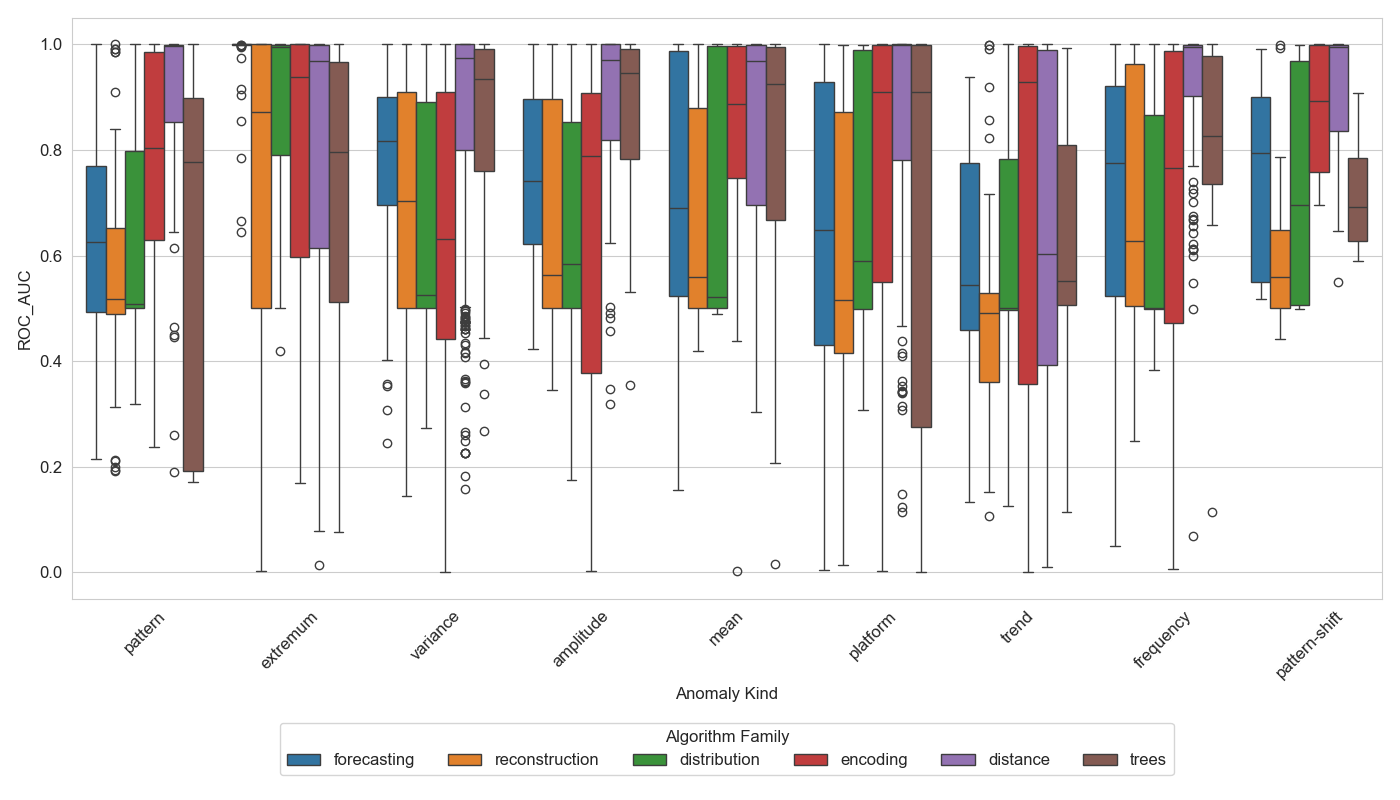
\includegraphics[width=1\textwidth]{plots/h1_boxplot_results.png}
    \caption{AUC-ROC Scores by Algorithm Family and Dataset}
    \label{fig:h1_boxplot_results}
\end{figure}

\begin{table}
\centering
\caption{Exact Values from Figure \ref{fig:h1_boxplot_results} with Mean Performance $> 0.8$}
\label{tab:best-performer}
\begin{tabular}{llrrr}
\toprule
 &  & count & mean & std \\
Anomaly Kind & Algorithm Family &  &  &  \\
\midrule
\multirow[t]{2}{*}{\textbf{amplitude}} & \textbf{distance} & 42 & 0.86 & 0.20 \\
\textbf{} & \textbf{trees} & 8 & 0.83 & 0.25 \\
\cline{1-5}
\multirow[t]{2}{*}{\textbf{extremum}} & \textbf{distribution} & 36 & 0.87 & 0.21 \\
\textbf{} & \textbf{forecasting} & 84 & 0.98 & 0.06 \\
\cline{1-5}
\multirow[t]{2}{*}{\textbf{frequency}} & \textbf{distance} & 125 & 0.92 & 0.14 \\
\textbf{} & \textbf{trees} & 24 & 0.83 & 0.20 \\
\cline{1-5}
\multirow[t]{2}{*}{\textbf{mean}} & \textbf{distance} & 82 & 0.85 & 0.20 \\
\textbf{} & \textbf{encoding} & 23 & 0.82 & 0.24 \\
\cline{1-5}
\textbf{pattern} & \textbf{distance} & 97 & 0.91 & 0.17 \\
\cline{1-5}
\multirow[t]{2}{*}{\textbf{pattern-shift}} & \textbf{distance} & 20 & 0.91 & 0.13 \\
\textbf{} & \textbf{encoding} & 6 & 0.87 & 0.14 \\
\cline{1-5}
\textbf{platform} & \textbf{distance} & 102 & 0.85 & 0.25 \\
\cline{1-5}
\multirow[t]{2}{*}{\textbf{variance}} & \textbf{distance} & 625 & 0.87 & 0.19 \\
\textbf{} & \textbf{trees} & 120 & 0.86 & 0.16 \\
\cline{1-5}
\bottomrule
\end{tabular}
\end{table}


Figure \ref{fig:h1_boxplot_results} reveals that there are differences in the mean performance values along different algorithm families per anomaly kind. Table \ref{tab:best-performer} shows the algorithm families with a mean performance value $>0.8$. We note that none of the algorithm families achieved this mean performance threshold on trend anomalies. The maximal mean performance on trend anomalies of $\sim 0.66$ was achieved by, both, distance and encoding algorithms.

The analysis highlights that distance-based methods stand out for their versatility, performing well across various anomaly types. This benefit is especially visible when capturing shifts in value and recurring patterns. 
Forecasting methods excel in extremum anomalies, showing the strengths of predictive models for significant deviations, such as sudden peaks or troughs. 
Tree methods are notably effective in handling amplitude, frequency and variance changes, while distribution-based methods perform best with extremum anomalies. Overall, distance-based methods provide robust, general performance, while other families like forecasting and distribution excel in more specific anomaly detection scenarios.

This analysis can already guide the choice of algorithms based on the specific anomaly types. Selecting algorithms from these families according to the anomaly kinds can yield optimized results in AD tasks on time series. However, Table \ref{tab:best-performer} shows variations in the standard deviation across all families, which asks for a deep-dive analysis within the families.


\section{Deep-Dive and Algorithm Analysis}
For each anomaly kind, we take a closer look at the performance results of each algorithm. The standard deviation in Figure \ref{fig:h1_boxplot_results} already revealed that within a best-performing family, some algorithms show bad performance. In the following, all algorithms within a best-performing family are compared to identify reasons why they outperformed or underperformed on a given anomaly kind. These results are formulated as hypotheses for internal structural advantages towards anomaly kinds. 

With distance methods being very prominent in this analysis, we first separate them further by their inherent structures and approaches to AD. The grouping in Table \ref{tab:distance_algos_structures} helps to simplify the analysis and retains a good overview.

\begin{table}[h!]
\centering
\caption{Grouping of Distance Algorithms by Structural Approach}
\label{tab:distance_algos_structures}
\begin{tabular}{ll}
\hline
\textbf{Structure/Approach} & \textbf{Algorithms} \\ \hline
\textbf{Model-Based} & NormA, SAND, SSA \\ 
\textbf{Symbolic and Pattern-Based} & HOT SAX, VALMOD \\
\textbf{Matrix Profile and Similarity-Based} & Left STAMPi, STOMP, STAMP \\
\textbf{Graph and Embedding-Based} & Series2Graph \\ 
\textbf{Density-Based} & Subsequence LOF \\ 
\textbf{SVM-Based and Hybrid Approaches} & PhaseSpace-SVM \\ \hline
\end{tabular}
\end{table}


\begin{itemize}
    \item \textbf{Model-Based}: Builds a model representing normal behavior, either through a predefined model (NormA) or adaptive, streaming updates (SAND, SSA). These algorithms detect anomalies as deviations from expected patterns.
    \item \textbf{Symbolic and Pattern-Based}: Utilizes symbolic representations or variable-length pattern recognition to identify unique or recurring subsequences. These methods focus on pattern distinctiveness and sometimes abstract details of fine variations.
    \item \textbf{Matrix Profile and Similarity-Based}: Employs matrix profiles to efficiently compute similarity joins. This structure allows to captures exact or near-exact patterns across large datasets.
    \item \textbf{Graph and Embedding-Based}: Represents time series data as a graph where nodes represent subsequences and edges indicate pattern transitions. 
    \item \textbf{Density-Based}: Detects anomalies based on local density measurements, identifying points that are isolated from their nearest neighbors.
    \item \textbf{SVM-Based and Hybrid Approaches}: Combines support vector machines with phase-space reconstruction to identify anomalies in temporal sequences, focusing on dynamic and nonlinear behaviors in time series data.
\end{itemize}


\subsection{Extremum Anomalies} 
    \begin{table}
\caption{Algorithms on extremum Anomaly within best-performing Family}
\label{tab:bp-extremum}
\begin{tabular}{llrrr}
\toprule
 &  & count & mean & std \\
Algorithm Family & Algorithm &  &  &  \\
\midrule
\multirow[t]{3}{*}{\textbf{distribution}} & \textbf{DSPOT} & 12 & 0.83 & 0.23 \\
\textbf{} & \textbf{DWT-MLEAD} & 12 & 0.94 & 0.11 \\
\textbf{} & \textbf{S-H-ESD (Twitter)} & 12 & 0.83 & 0.25 \\
\cline{1-5}
\multirow[t]{7}{*}{\textbf{forecasting}} & \textbf{ARIMA} & 12 & 0.89 & 0.13 \\
\textbf{} & \textbf{MedianMethod} & 12 & 1.00 & 0.00 \\
\textbf{} & \textbf{NumentaHTM} & 12 & 1.00 & 0.00 \\
\textbf{} & \textbf{OceanWNN} & 12 & 1.00 & 0.00 \\
\textbf{} & \textbf{Random Forest Regressor (RR)} & 12 & 1.00 & 0.00 \\
\textbf{} & \textbf{Triple ES (Holt-Winter's)} & 12 & 1.00 & 0.00 \\
\textbf{} & \textbf{XGBoosting (RR)} & 12 & 1.00 & 0.00 \\
\cline{1-5}
\bottomrule
\end{tabular}
\end{table}

    \textit{Forecasting} almost detected all extremum anomalies in testing, with ARIMA only missing a few.
    The adaptability to dynamic patterns of the MedianMethod, NumentaHTM and OceanWNN as well as the robustness through ensemble learning of RForest and XGBoosting seem to favor the detection of extremum anomalies. 
    ARIMA might struggle with non-linear or abrupt changes, which are typical in extremum anomalies. Its reliance on linear assumptions could limit its precision on complex, non-linear data patterns.
    
    \textit{Distribution} algorithms also performed reasonably well on extremum anomalies. DWT-MLEAD shows the best performance with highest consistency. The breakdown of the time series into multiple frequency components allows DWT-MLEAD to capture both short-term spikes and broader extremum patterns effectively, reflecting in the good overall performance. By additionally applying MLE on the decomposed data, DWT-MLEAD optimizes its thresholding, which likely reduces false positives (shown in its lower std dev of 0.11).
    DSPOT's dynamic threshold, being optimized for streaming data, adapts quickly. This might lead to a high sensitivity. Additionally, it does not decompose at multiple scales but instead applies its threshold across the entire dataset. If noise or frequent fluctuations are present, DSPOT might mistakenly classify these as extremum points, impacting its overall precision.
    S-H-ESD is robust to seasonality, which might make it less effective for unpredictable extremum anomalies that fall outside seasonal expectations.

\subsection{Frequency Anomalies}
    \begin{table}
\caption{Algorithms on frequency Anomaly within best-performing Family}
\label{tab:bp-frequency}
\begin{tabular}{llrrrrrrrr}
\toprule
 &  & count & mean & std & min & 25\% & 50\% & 75\% & max \\
Algorithm Family & Algorithm &  &  &  &  &  &  &  &  \\
\midrule
\multirow[t]{11}{*}{\textbf{distance}} & \textbf{HOT SAX} & 5.00 & 0.80 & 0.20 & 0.50 & 0.73 & 0.83 & 0.97 & 1.00 \\
\textbf{} & \textbf{Left STAMPi} & 12.00 & 0.98 & 0.04 & 0.89 & 0.98 & 1.00 & 1.00 & 1.00 \\
\textbf{} & \textbf{NormA} & 12.00 & 1.00 & 0.01 & 0.98 & 1.00 & 1.00 & 1.00 & 1.00 \\
\textbf{} & \textbf{PhaseSpace-SVM} & 12.00 & 0.95 & 0.06 & 0.82 & 0.90 & 0.99 & 1.00 & 1.00 \\
\textbf{} & \textbf{SAND} & 12.00 & 0.99 & 0.01 & 0.97 & 0.99 & 1.00 & 1.00 & 1.00 \\
\textbf{} & \textbf{SSA} & 12.00 & 0.71 & 0.14 & 0.55 & 0.61 & 0.66 & 0.76 & 1.00 \\
\textbf{} & \textbf{STAMP} & 12.00 & 0.97 & 0.06 & 0.81 & 0.98 & 1.00 & 1.00 & 1.00 \\
\textbf{} & \textbf{STOMP} & 12.00 & 0.97 & 0.06 & 0.81 & 0.98 & 1.00 & 1.00 & 1.00 \\
\textbf{} & \textbf{Series2Graph} & 12.00 & 0.87 & 0.27 & 0.07 & 0.89 & 0.99 & 1.00 & 1.00 \\
\textbf{} & \textbf{Subsequence LOF} & 12.00 & 0.94 & 0.13 & 0.67 & 0.99 & 1.00 & 1.00 & 1.00 \\
\textbf{} & \textbf{VALMOD} & 12.00 & 0.90 & 0.15 & 0.61 & 0.80 & 0.99 & 1.00 & 1.00 \\
\cline{1-10}
\multirow[t]{2}{*}{\textbf{trees}} & \textbf{PST} & 12.00 & 0.92 & 0.11 & 0.66 & 0.93 & 0.97 & 0.99 & 1.00 \\
\textbf{} & \textbf{Subsequence IF} & 12.00 & 0.73 & 0.22 & 0.11 & 0.73 & 0.75 & 0.77 & 1.00 \\
\cline{1-10}
\bottomrule
\end{tabular}
\end{table}

    Within the \textit{distance} family, two model-based methods NormA and SAND achieved the highest means ($0.997$ and $0.993$) with very low variance. However, SSA yields the lowest performance of all distance methods. This does not generally speak in favor of model-based structures towards frequency anomalies, but, SSA is build around seasonal and trend components. It might overly rely on these components, leading to bad performance in frequency anomalies.
    The matrix-profile and similarity based approaches overall show high mean performance with small standard deviations. This inherent structure excels at identifying repeated sequences, probably leading to the high performance on frequency anomalies.
    The rest shows moderate to high performance with no indication on structural advantages.
    
    PST from the \textit{tree} family achieves comparable results. It likely outperforms Subsequence IF due to its focuses on encoding frequent patterns with suffix trees. By capturing these patterns probabilistically, it is better suited to recognize anomalies as any deviation in the frequency of expected patterns, which is ideal for detecting frequency anomalies. Subsequence IF does not inherently focus on frequency anomalies but isolates points independently, which may produce false positives or miss certain frequency-related anomalies.
    
\subsection{Mean Anomalies} 
    \begin{table}[h]
\centering
\caption{Algorithms on Mean Anomaly within best-performing Family}
\label{tab:bp-mean}
\begin{tabular}{llrrr}
\toprule
 &  & count & mean & std \\
Algorithm Family & Algorithm &  &  &  \\
\midrule
\multirow[t]{11}{*}{\textbf{distance}} & \textbf{HOT SAX} & 3 & 0.85 & 0.21 \\
\textbf{} & \textbf{Left STAMPi} & 8 & 0.83 & 0.28 \\
\textbf{} & \textbf{NormA} & 8 & 0.88 & 0.23 \\
\textbf{} & \textbf{PhaseSpace-SVM} & 8 & 0.73 & 0.17 \\
\textbf{} & \textbf{SAND} & 7 & 0.96 & 0.05 \\
\textbf{} & \textbf{SSA} & 8 & 0.80 & 0.16 \\
\textbf{} & \textbf{STAMP} & 8 & 0.90 & 0.24 \\
\textbf{} & \textbf{STOMP} & 8 & 0.90 & 0.24 \\
\textbf{} & \textbf{Series2Graph} & 8 & 0.92 & 0.12 \\
\textbf{} & \textbf{Subsequence LOF} & 8 & 0.94 & 0.09 \\
\textbf{} & \textbf{VALMOD} & 8 & 0.67 & 0.20 \\
\cline{1-5}
\multirow[t]{3}{*}{\textbf{encoding}} & \textbf{GrammarViz} & 8 & 0.98 & 0.04 \\
\textbf{} & \textbf{TARZAN} & 7 & 0.70 & 0.37 \\
\textbf{} & \textbf{TSBitmap} & 8 & 0.77 & 0.14 \\
\cline{1-5}
\bottomrule
\end{tabular}
\end{table}

    Looking back at Table \ref{tab:best-performer} we see only a small difference, between the two best-performing families distance and encoding, on mean anomalies.
    Overall, the \textit{distance} family does not show a high variablilty in performance between different algorithms. All algorithms show moderate to high performance mean with PhaseSpace-SVM and VALMOD being the exception. This does not align with the structural grouping from Table \ref{tab:distance_algos_structures} and needs further analysis of the two algorithms. Both PhaseSpace-SVM and VALMOD are optimized for detecting distinct or abrupt anomalies tied to structural or temporal patterns rather than gradual shifts in central tendency. PhaseSpace-SVM focuses on temporal evolution, making it more suited to dynamic anomalies, while VALMOD searches distinctive motifs or isolated discords. Both approaches do not align well with the characteristics of mean anomalies.
    
    A similar concept could explain the deviations in the \textit{encoding} family. GrammarViz clearly outperforms TARZAN and TSBitmap. GrammarViz’s identifies deviations from common rules, its grammar, which makes it well-suited for detecting gradual changes in central tendency. TARZAN uses a suffix tree combined with a Markov model to detect surprising patterns, while TSBitmap focuses on visual pattern detection. Both approaches might hinder the performance on gradual changes.
    
\subsection{Pattern Anomalies}
    \begin{table}
\caption{Algorithms on pattern Anomaly within best-performing Family}
\label{tab:bp-pattern}
\begin{tabular}{llrrr}
\toprule
 &  & count & mean & std \\
Algorithm Family & Algorithm &  &  &  \\
\midrule
\multirow[t]{11}{*}{\textbf{distance}} & \textbf{HOT SAX} & 7 & 0.76 & 0.30 \\
\textbf{} & \textbf{Left STAMPi} & 9 & 0.95 & 0.10 \\
\textbf{} & \textbf{NormA} & 9 & 0.96 & 0.10 \\
\textbf{} & \textbf{PhaseSpace-SVM} & 9 & 0.90 & 0.13 \\
\textbf{} & \textbf{SAND} & 9 & 0.96 & 0.08 \\
\textbf{} & \textbf{SSA} & 9 & 0.79 & 0.28 \\
\textbf{} & \textbf{STAMP} & 9 & 0.94 & 0.12 \\
\textbf{} & \textbf{STOMP} & 9 & 0.94 & 0.12 \\
\textbf{} & \textbf{Series2Graph} & 9 & 0.92 & 0.18 \\
\textbf{} & \textbf{Subsequence LOF} & 9 & 0.97 & 0.05 \\
\textbf{} & \textbf{VALMOD} & 9 & 0.86 & 0.20 \\
\cline{1-5}
\bottomrule
\end{tabular}
\end{table}

    Distance based approaches appear to capture pattern anomalies the best, with most  algorithms achieving high performance results. SSA and HOT SAX strike with lower mean performance and the highest standard deviation.
    With VALMOD performing well but also lower than average (mean of $0.91$ across all anomaly kinds) symbolic and pattern-based approaches appear to underperform on pattern anomalies, contrary to their original idea. Depending on the scale of abnormality, this could be explained by their level of abstraction, which can lead to a lower sensitivity.
    The bad performance of SSA could, again, be explained by its assumption of inherent seasonal and trend components.
    
\subsection{Pattern Shift Anomalies}
    \begin{table}
\caption{Algorithms on pattern-shift Anomaly within best-performing Family}
\label{tab:bp-pattern-shift}
\begin{tabular}{llrrr}
\toprule
 &  & count & mean & std \\
Algorithm Family & Algorithm &  &  &  \\
\midrule
\multirow[t]{10}{*}{\textbf{distance}} & \textbf{Left STAMPi} & 2 & 1.00 & 0.00 \\
\textbf{} & \textbf{NormA} & 2 & 1.00 & 0.00 \\
\textbf{} & \textbf{PhaseSpace-SVM} & 2 & 0.84 & 0.04 \\
\textbf{} & \textbf{SAND} & 2 & 1.00 & 0.00 \\
\textbf{} & \textbf{SSA} & 2 & 0.73 & 0.26 \\
\textbf{} & \textbf{STAMP} & 2 & 1.00 & 0.00 \\
\textbf{} & \textbf{STOMP} & 2 & 1.00 & 0.00 \\
\textbf{} & \textbf{Series2Graph} & 2 & 0.82 & 0.25 \\
\textbf{} & \textbf{Subsequence LOF} & 2 & 0.84 & 0.05 \\
\textbf{} & \textbf{VALMOD} & 2 & 0.83 & 0.01 \\
\cline{1-5}
\multirow[t]{3}{*}{\textbf{encoding}} & \textbf{GrammarViz} & 2 & 1.00 & 0.00 \\
\textbf{} & \textbf{TARZAN} & 2 & 0.85 & 0.21 \\
\textbf{} & \textbf{TSBitmap} & 2 & 0.77 & 0.03 \\
\cline{1-5}
\bottomrule
\end{tabular}
\end{table}

    Here, the \textit{distance} family shows a similar picture. SSA seems to struggle with handling pattern-shift anomalies due to missing seasonal and trend components, while the other model-based approaches outperform.
    Matrix profile and similarity based algorithms excel on pattern-shift anomalies. As they can continuously compare subsequences across the time series they are sensitivity to changes in similarity allowing them to effectively catch pattern shifts.

    For \textit{encoding} algorithms, we follow the hypothesis formulated for mean anomalies, to explain the bad performance of TARZAN and TSBitmap. The same goes for GrammarViz. Its established grammar is broken by pattern shifts, which introduce deviations in sequence or timing, probably making it efficient on pattern-shifts.
    
\subsection{Platform Anomalies}
    \begin{table}[h]
\centering
\caption{Algorithms on Platform Anomaly within best-performing Family}
\label{tab:bp-platform}
\begin{tabular}{llrrr}
\toprule
 &  & count & mean & std \\
Algorithm Family & Algorithm &  &  &  \\
\midrule
\multirow[t]{11}{*}{\textbf{distance}} & \textbf{HOT SAX} & 5 & 0.76 & 0.35 \\
\textbf{} & \textbf{Left STAMPi} & 10 & 0.93 & 0.21 \\
\textbf{} & \textbf{NormA} & 10 & 0.91 & 0.20 \\
\textbf{} & \textbf{PhaseSpace-SVM} & 10 & 0.83 & 0.28 \\
\textbf{} & \textbf{SAND} & 10 & 0.93 & 0.15 \\
\textbf{} & \textbf{SSA} & 10 & 0.67 & 0.27 \\
\textbf{} & \textbf{STAMP} & 10 & 0.93 & 0.21 \\
\textbf{} & \textbf{STOMP} & 10 & 0.93 & 0.21 \\
\textbf{} & \textbf{Series2Graph} & 9 & 0.82 & 0.34 \\
\textbf{} & \textbf{Subsequence LOF} & 10 & 0.69 & 0.23 \\
\textbf{} & \textbf{VALMOD} & 8 & 0.92 & 0.23 \\
\cline{1-5}
\bottomrule
\end{tabular}
\end{table}

    Model-based and matrix profile and similarity-based algorithms show high performance throughout, with SSA being the exception possible due to the missing trend and seasonality components.
    Almost all other approaches only achieve moderate performance on platform anomalies. Strikingly, VALMOD achieves good performance with moderate standard deviation within the rest. In platform anomalies, where the data holds a new baseline over a prolonged period, the motif and discord discovery might capture the new levels in the time series as distinct patterns. This could be seen as a structural advantage on platform anomalies.
    
\subsection{Variance Anomalies}
    \begin{table}
\caption{Algorithms on variance Anomaly within best-performing Family}
\label{tab:bp-variance}
\begin{tabular}{llrrr}
\toprule
 &  & count & mean & std \\
Algorithm Family & Algorithm &  &  &  \\
\midrule
\multirow[t]{11}{*}{\textbf{distance}} & \textbf{HOT SAX} & 47 & 0.78 & 0.20 \\
\textbf{} & \textbf{Left STAMPi} & 60 & 0.89 & 0.16 \\
\textbf{} & \textbf{NormA} & 50 & 0.72 & 0.25 \\
\textbf{} & \textbf{PhaseSpace-SVM} & 60 & 0.97 & 0.05 \\
\textbf{} & \textbf{SAND} & 49 & 0.88 & 0.17 \\
\textbf{} & \textbf{SSA} & 60 & 0.75 & 0.21 \\
\textbf{} & \textbf{STAMP} & 60 & 0.90 & 0.17 \\
\textbf{} & \textbf{STOMP} & 60 & 0.90 & 0.17 \\
\textbf{} & \textbf{Series2Graph} & 59 & 0.87 & 0.17 \\
\textbf{} & \textbf{Subsequence LOF} & 60 & 0.97 & 0.07 \\
\textbf{} & \textbf{VALMOD} & 60 & 0.91 & 0.16 \\
\cline{1-5}
\multirow[t]{2}{*}{\textbf{trees}} & \textbf{PST} & 60 & 0.87 & 0.18 \\
\textbf{} & \textbf{Subsequence IF} & 60 & 0.86 & 0.15 \\
\cline{1-5}
\bottomrule
\end{tabular}
\end{table}

    The \textit{distance} family reveals a different picture on variance anomalies. While performing well on other anomaly types, NormA marks the worst mean performance value here. The reason might be its reliance on detecting changes in the central tendency. Changes in data spread, like variance anomalies, do not align with this focus, thus, potentially leading to the bad performance.
    PhaceSpace-SVM, on the other hand, achieves a higher performance than its mean across all anomaly kinds. Its phase-space reconstruction seems to captures dynamic, variance-based changes in data more reliably than a stable central model. The SVM possibly enhances this by identifying boundary deviations, which are characteristic of variance anomalies. 
    It has to be noted that, as indicated by the counts in Table \ref{tab:bp-variance} and seen in Figure \ref{fig:distribution_chart}, the most samples were used in the evaluation on this anomaly type.
    
\subsection{Trend Anomalies} 
    As noted above, none of the algorithm families achieved mean performance threshold on trend anomalies. We break our methodology to identify best-performers across all families.
    \begin{table}[h]
\centering
\caption{Individual Algorithm Performance Analysis on Trend Anomalies.}
\label{tab:bp-trend}
\begin{tabular}{llrrr}
\toprule
 &  & count & mean & std \\
Algorithm Family & Algorithm &  &  &  \\
\midrule
\textbf{distance} & \textbf{Subsequence LOF} & 5.00 & 0.86 & 0.29 \\
\cline{1-5}
\textbf{distribution} & \textbf{DWT-MLEAD} & 5.00 & 0.82 & 0.39 \\
\cline{1-5}
\multirow[t]{2}{*}{\textbf{encoding}} & \textbf{GrammarViz} & 5.00 & 0.91 & 0.21 \\
\textbf{} & \textbf{TSBitmap} & 5.00 & 0.83 & 0.28 \\
\cline{1-5}
\bottomrule
\end{tabular}
\end{table}
    Table \ref{tab:bp-trend} reveals that encoding methods perform well on trend anomalies but were not considered because of the destructive performance result of TARZAN of $0.13$. This significant difference in the performance results within one family can be explained by TARZAN's inherent focus on discrete, unexpected patterns. GrammarViz’s grammar-based approach detects shifts in established patterns, while TSBitmap’s visual representation highlights progressive changes. A similar focus that is set by Subsequence LOF, which together make up the highest mean performance values on trend anomalies. 
    Interestingly, SSA only achieved a mean performance of $0.65$ on trend anomalies, which is incompatible with our hypothesis that it excels on time series with trend and seasonal components. 



% Challenges and Solutions
% Code Snippets 
\chapter{Implementing an Expert System}
\label{ch:implementing_an_expert_system}
% Implementation Steps
1. Using GutenTAG for feature extraction

1.1 Feature extraction per algo family

1.1.1 Running tsfresh feature extraction on small subset of data (20 instances per algorithm family) to prefilter relevant features (relevant = correlation between feature and algo family AUC ROC). Argument that feature extraction is very computationally intensive "could not get it to work altough njobs npartitions", so had to drop some features (list)
Christ et al. have shown that adjusting the list of calculated features changes the total runtime of feature extraction drastically. In addition, they deliver average runtime results for one time series with 1000 time steps for all used feature extraction methods \cite{tsfresh}. We follow these findings and eliminate the three feature extraction methods with an average runtime per time series $>1 s$ to boost calculation.
tsfresh is very computationally expensive. A hurdle many researchers struggeled with. Couldn't get extraction of reduced feature set running on server for all samples ref Graph with sample size (memory error see txt file 86.6 TiB).
200 samples also didn't work. Same error
150 samples also didn't work. Same error
Also tried to run each group (algo family) individually to reduce system load -> same error
Trying to run features >0.4 correlation coeff

1.1.2 Running feature extraction of prefiltered features on bigger dataset

1.1.3 Analyze differences in features from small to bigger subset
We reached consistency; now all features with correlation >0.4 for whole dataset

1.1.4 Analyze correlation algo family to features per algo family

1.2 Feature extraction per anomaly type (on num samples computed in above evaluation?)

1.3 Feature extraction on all Datasets used in the eval paper

%\section{Experiment Setup}
% Beschreibung der Experimentanordnung und der technischen Details.


\chapter{Results}
This is a summary of the results from Chapter \ref{ch:identifying_best_performers} and \ref{ch:implementing_an_expert_system}.

\section{Best Performers}
\begin{itemize}
    \item From Data Analysis
    \item Map to Theory/ Literature Review and Structures of Algorithms
\end{itemize}

% 2. If there is a correlation, identify possible reasons, why some algos perform better on certain anomaly types
%A significant correlation shows that the detection capabilities depend on the anomaly type to detect and the method algorithms use to detect it. Following this finding we can formulate hypotheses on what characteristics are beneficial for detecting certain anomaly types. 
% 3. dive deeper and analyze the differences in characteristics and performance within one group + Proof that the these algo characteristics are the reason for their performance benefit (how?).
%Since there are also structural differences between algortihms within one family, a deeper dive into each family and the including algorithms is performed. Potential deviations in performance within one family could rule out unnecessary characteristics and ultimately identify beneficial characteristics. A performance comparison between similar algorithms that differ in the identified characteristic could help to proof that the performance increase is due to this certain characteristic.

\section{Expert System}
\begin{itemize}
    \item Feature Selection
    \item Bewertung der Performance anhand relevanter Metriken und Vergleich mit Baselines\todo{include "good" model characteristics from survey}
\end{itemize}

\section{Discussion of Results}
\begin{itemize}
    \item Interpretation der Ergebnisse und deren Implikationen
    \item Diskussion der Stärken und Schwächen.
\end{itemize}


\chapter{Conclusion}
% Summary of Findings
\begin{itemize}
    \item Algorithms should only be evaluated on the discovered anomaly type and compared within their family to solve the problem of comparability
    \item We suggest the mapping of algorithm families to anomaly types as a solution to the problem of performance comparison presented by Braei et al. \cite{Braei2020}.
    \item The better solution is different algorithms for different anomaly types -> expert system
    \item only tested on GutenTAG, might be biased, good to test on other dataset that offers unique anomalies
    \item Ergebnisse auch sehr parameter abhängig, besonders bei sensitiven algorithmen
    \item Weg von time series, was gibts noch
    % Future Work
    \item Extend to supervised, another prefilter if labels are available
    including potential extensions to more complex multivariate settings
    model compression for real-time applications
\end{itemize}

% Include more chapters here

\appendix
% Include appendices here
\chapter{Appendix}
\todo{page: ich hab die Inhalte selbst erstellt}
\todo{page: Textuelle veränderungen wurden mit LLMs gemacht, in Absprache mit Betreuer}
Some important source texts are listed in this appendix.
\todo{Hardwaresetup Server auflisten}

\begin{lstlisting}
public class Hello {
    public static void main(String[] args) {
        System.out.println("Hello World");
    }
}
\end{lstlisting}

\begin{tabular}{|l|l|c|c|c|c|c|c|c|c|}
\toprule
 &  & count & mean & std & min & 25\% & 50\% & 75\% & max \\
anomaly_kind & algo_family &  &  &  &  &  &  &  &  \\
\midrule
\multirow[t]{6}{*}{amplitude} & distance & 42 & 0.860000 & 0.200000 & 0.320000 & 0.820000 & 0.970000 & 1.000000 & 1.000000 \\
 & distribution & 12 & 0.660000 & 0.250000 & 0.180000 & 0.500000 & 0.580000 & 0.850000 & 1.000000 \\
 & encoding & 12 & 0.650000 & 0.360000 & 0.000000 & 0.380000 & 0.790000 & 0.910000 & 1.000000 \\
 & forecasting & 28 & 0.740000 & 0.170000 & 0.420000 & 0.620000 & 0.740000 & 0.900000 & 1.000000 \\
 & reconstruction & 28 & 0.650000 & 0.210000 & 0.340000 & 0.500000 & 0.560000 & 0.900000 & 1.000000 \\
 & trees & 8 & 0.830000 & 0.250000 & 0.350000 & 0.780000 & 0.950000 & 0.990000 & 1.000000 \\
\cline{1-10}
\multirow[t]{6}{*}{extremum} & distance & 132 & 0.800000 & 0.270000 & 0.010000 & 0.620000 & 0.970000 & 1.000000 & 1.000000 \\
 & distribution & 36 & 0.870000 & 0.210000 & 0.420000 & 0.790000 & 1.000000 & 1.000000 & 1.000000 \\
 & encoding & 24 & 0.780000 & 0.280000 & 0.170000 & 0.600000 & 0.940000 & 1.000000 & 1.000000 \\
 & forecasting & 84 & 0.980000 & 0.060000 & 0.650000 & 1.000000 & 1.000000 & 1.000000 & 1.000000 \\
 & reconstruction & 84 & 0.720000 & 0.310000 & 0.000000 & 0.500000 & 0.870000 & 1.000000 & 1.000000 \\
 & trees & 24 & 0.690000 & 0.320000 & 0.080000 & 0.510000 & 0.800000 & 0.970000 & 1.000000 \\
\cline{1-10}
\multirow[t]{6}{*}{frequency} & distance & 125 & 0.920000 & 0.140000 & 0.070000 & 0.900000 & 1.000000 & 1.000000 & 1.000000 \\
 & distribution & 36 & 0.650000 & 0.220000 & 0.380000 & 0.500000 & 0.500000 & 0.870000 & 1.000000 \\
 & encoding & 36 & 0.680000 & 0.340000 & 0.010000 & 0.470000 & 0.770000 & 0.990000 & 1.000000 \\
 & forecasting & 84 & 0.720000 & 0.200000 & 0.050000 & 0.520000 & 0.770000 & 0.920000 & 1.000000 \\
 & reconstruction & 84 & 0.700000 & 0.210000 & 0.250000 & 0.500000 & 0.630000 & 0.960000 & 1.000000 \\
 & trees & 24 & 0.830000 & 0.200000 & 0.110000 & 0.730000 & 0.830000 & 0.980000 & 1.000000 \\
\cline{1-10}
\multirow[t]{6}{*}{mean} & distance & 82 & 0.850000 & 0.200000 & 0.300000 & 0.700000 & 0.970000 & 1.000000 & 1.000000 \\
 & distribution & 24 & 0.700000 & 0.240000 & 0.490000 & 0.500000 & 0.520000 & 1.000000 & 1.000000 \\
 & encoding & 23 & 0.820000 & 0.240000 & 0.000000 & 0.750000 & 0.890000 & 1.000000 & 1.000000 \\
 & forecasting & 56 & 0.740000 & 0.240000 & 0.160000 & 0.520000 & 0.690000 & 0.990000 & 1.000000 \\
 & reconstruction & 56 & 0.670000 & 0.200000 & 0.420000 & 0.500000 & 0.560000 & 0.880000 & 1.000000 \\
 & trees & 16 & 0.790000 & 0.300000 & 0.020000 & 0.670000 & 0.920000 & 0.990000 & 1.000000 \\
\cline{1-10}
\multirow[t]{6}{*}{pattern} & distance & 97 & 0.910000 & 0.170000 & 0.190000 & 0.850000 & 1.000000 & 1.000000 & 1.000000 \\
 & distribution & 26 & 0.610000 & 0.180000 & 0.320000 & 0.500000 & 0.510000 & 0.800000 & 1.000000 \\
 & encoding & 27 & 0.760000 & 0.240000 & 0.240000 & 0.630000 & 0.800000 & 0.990000 & 1.000000 \\
 & forecasting & 63 & 0.630000 & 0.180000 & 0.220000 & 0.490000 & 0.630000 & 0.770000 & 1.000000 \\
 & reconstruction & 63 & 0.580000 & 0.200000 & 0.190000 & 0.490000 & 0.520000 & 0.650000 & 1.000000 \\
 & trees & 18 & 0.620000 & 0.340000 & 0.170000 & 0.190000 & 0.780000 & 0.900000 & 1.000000 \\
\cline{1-10}
\multirow[t]{6}{*}{pattern-shift} & distance & 20 & 0.910000 & 0.130000 & 0.550000 & 0.840000 & 1.000000 & 1.000000 & 1.000000 \\
 & distribution & 6 & 0.730000 & 0.250000 & 0.500000 & 0.510000 & 0.700000 & 0.970000 & 1.000000 \\
 & encoding & 6 & 0.870000 & 0.140000 & 0.700000 & 0.760000 & 0.890000 & 1.000000 & 1.000000 \\
 & forecasting & 14 & 0.750000 & 0.190000 & 0.520000 & 0.550000 & 0.790000 & 0.900000 & 0.990000 \\
 & reconstruction & 14 & 0.630000 & 0.180000 & 0.440000 & 0.500000 & 0.560000 & 0.650000 & 1.000000 \\
 & trees & 4 & 0.720000 & 0.140000 & 0.590000 & 0.630000 & 0.690000 & 0.780000 & 0.910000 \\
\cline{1-10}
\multirow[t]{6}{*}{platform} & distance & 102 & 0.850000 & 0.250000 & 0.110000 & 0.780000 & 1.000000 & 1.000000 & 1.000000 \\
 & distribution & 30 & 0.710000 & 0.240000 & 0.310000 & 0.500000 & 0.590000 & 0.990000 & 1.000000 \\
 & encoding & 29 & 0.720000 & 0.360000 & 0.000000 & 0.550000 & 0.910000 & 1.000000 & 1.000000 \\
 & forecasting & 70 & 0.650000 & 0.290000 & 0.000000 & 0.430000 & 0.650000 & 0.930000 & 1.000000 \\
 & reconstruction & 70 & 0.570000 & 0.310000 & 0.010000 & 0.420000 & 0.510000 & 0.870000 & 1.000000 \\
 & trees & 20 & 0.680000 & 0.380000 & 0.000000 & 0.280000 & 0.910000 & 1.000000 & 1.000000 \\
\cline{1-10}
\multirow[t]{6}{*}{trend} & distance & 51 & 0.660000 & 0.320000 & 0.010000 & 0.390000 & 0.600000 & 0.990000 & 1.000000 \\
 & distribution & 15 & 0.610000 & 0.260000 & 0.130000 & 0.500000 & 0.500000 & 0.780000 & 1.000000 \\
 & encoding & 14 & 0.660000 & 0.410000 & 0.000000 & 0.360000 & 0.930000 & 1.000000 & 1.000000 \\
 & forecasting & 35 & 0.580000 & 0.200000 & 0.130000 & 0.460000 & 0.540000 & 0.780000 & 0.940000 \\
 & reconstruction & 35 & 0.500000 & 0.240000 & 0.110000 & 0.360000 & 0.490000 & 0.530000 & 1.000000 \\
 & trees & 10 & 0.620000 & 0.270000 & 0.110000 & 0.510000 & 0.550000 & 0.810000 & 0.990000 \\
\cline{1-10}
\multirow[t]{6}{*}{variance} & distance & 625 & 0.870000 & 0.190000 & 0.160000 & 0.800000 & 0.970000 & 1.000000 & 1.000000 \\
 & distribution & 179 & 0.650000 & 0.210000 & 0.270000 & 0.500000 & 0.530000 & 0.890000 & 1.000000 \\
 & encoding & 169 & 0.640000 & 0.280000 & 0.000000 & 0.440000 & 0.630000 & 0.910000 & 1.000000 \\
 & forecasting & 420 & 0.790000 & 0.150000 & 0.240000 & 0.690000 & 0.820000 & 0.900000 & 1.000000 \\
 & reconstruction & 420 & 0.710000 & 0.210000 & 0.140000 & 0.500000 & 0.700000 & 0.910000 & 1.000000 \\
 & trees & 120 & 0.860000 & 0.160000 & 0.270000 & 0.760000 & 0.940000 & 0.990000 & 1.000000 \\
\cline{1-10}
\bottomrule
\end{tabular}

\begin{table}
\centering
\caption{Best-performing Algorithm's Mean Performance across all Anomaly Types.}
\label{tab:performance_across_anomaly_kinds}
\begin{tabular}{llr}
\toprule
 &  & mean \\
Algorithm Family & Algorithm &  \\
\midrule
\multirow[t]{11}{*}{\textbf{distance}} & \textbf{HOT SAX} & 0.66 \\
\textbf{} & \textbf{Left STAMPi} & 0.88 \\
\textbf{} & \textbf{NormA} & 0.84 \\
\textbf{} & \textbf{PhaseSpace-SVM} & 0.87 \\
\textbf{} & \textbf{SAND} & 0.90 \\
\textbf{} & \textbf{SSA} & 0.77 \\
\textbf{} & \textbf{STAMP} & 0.88 \\
\textbf{} & \textbf{STOMP} & 0.88 \\
\textbf{} & \textbf{Series2Graph} & 0.84 \\
\textbf{} & \textbf{Subsequence LOF} & 0.91 \\
\textbf{} & \textbf{VALMOD} & 0.80 \\
\cline{1-3}
\multirow[t]{3}{*}{\textbf{distribution}} & \textbf{DSPOT} & 0.56 \\
\textbf{} & \textbf{DWT-MLEAD} & 0.90 \\
\textbf{} & \textbf{S-H-ESD (Twitter)} & 0.60 \\
\cline{1-3}
\multirow[t]{3}{*}{\textbf{encoding}} & \textbf{GrammarViz} & 0.93 \\
\textbf{} & \textbf{TARZAN} & 0.47 \\
\textbf{} & \textbf{TSBitmap} & 0.73 \\
\cline{1-3}
\multirow[t]{7}{*}{\textbf{forecasting}} & \textbf{ARIMA} & 0.75 \\
\textbf{} & \textbf{MedianMethod} & 0.57 \\
\textbf{} & \textbf{NumentaHTM} & 0.65 \\
\textbf{} & \textbf{OceanWNN} & 0.78 \\
\textbf{} & \textbf{Random Forest Regressor (RR)} & 0.85 \\
\textbf{} & \textbf{Triple ES (Holt-Winter's)} & 0.67 \\
\textbf{} & \textbf{XGBoosting (RR)} & 0.85 \\
\cline{1-3}
\multirow[t]{7}{*}{\textbf{reconstruction}} & \textbf{Bagel} & 0.55 \\
\textbf{} & \textbf{Donut} & 0.85 \\
\textbf{} & \textbf{FFT} & 0.53 \\
\textbf{} & \textbf{ImageEmbeddingCAE} & 0.85 \\
\textbf{} & \textbf{PCI} & 0.61 \\
\textbf{} & \textbf{SR-CNN} & 0.50 \\
\textbf{} & \textbf{Spectral Residual (SR)} & 0.55 \\
\cline{1-3}
\multirow[t]{2}{*}{\textbf{trees}} & \textbf{PST} & 0.76 \\
\textbf{} & \textbf{Subsequence IF} & 0.72 \\
\cline{1-3}
\bottomrule
\end{tabular}
\end{table}



\backmatter

\printbibliography

\clearpage
\thispagestyle{empty}

Name: \fullname \hfill Matriculation Number: \matnr \vspace{2cm}

\minisec{Declaration}

I declare that I have written this thesis independently and have not used any sources or aids other than those specified.\vspace{2cm}

Ulm, \dotfill

\hspace{10cm} {\footnotesize \fullname}
\end{document}
